\chapter{Коэффициент усиления}
Даны 2 передаточные функции:
\[
W_1(s) = \frac{s-1}{s^2 + 6s + 7}
\]
\[
W_2(s) = \frac{10s^3 + 15s^2 + 18s + 6}{10s^3 -10s^2}
\]

Добавим к передаточным функциям коэффициент усиления $k$:
\[
W_1(s) = \frac{k(s-1)}{s^2 + 6s + 7}
\]
\[
W_2(s) = \frac{k(10s^3 + 15s^2 + 18s + 6)}{10s^3 -10s^2}
\]

\section{Передаточная функция $W_1(s)$}
Построим годограф Найквиста для передаточных функций с различными значениями коэффициента усиления $k$:
\begin{enumerate}
    \item $k = 1$:
    \item $k = 2$:
    \item $k = 5$:
    \item $k = 10$:
\end{enumerate}

\begin{figure}[H]
    \centering
    \centering
    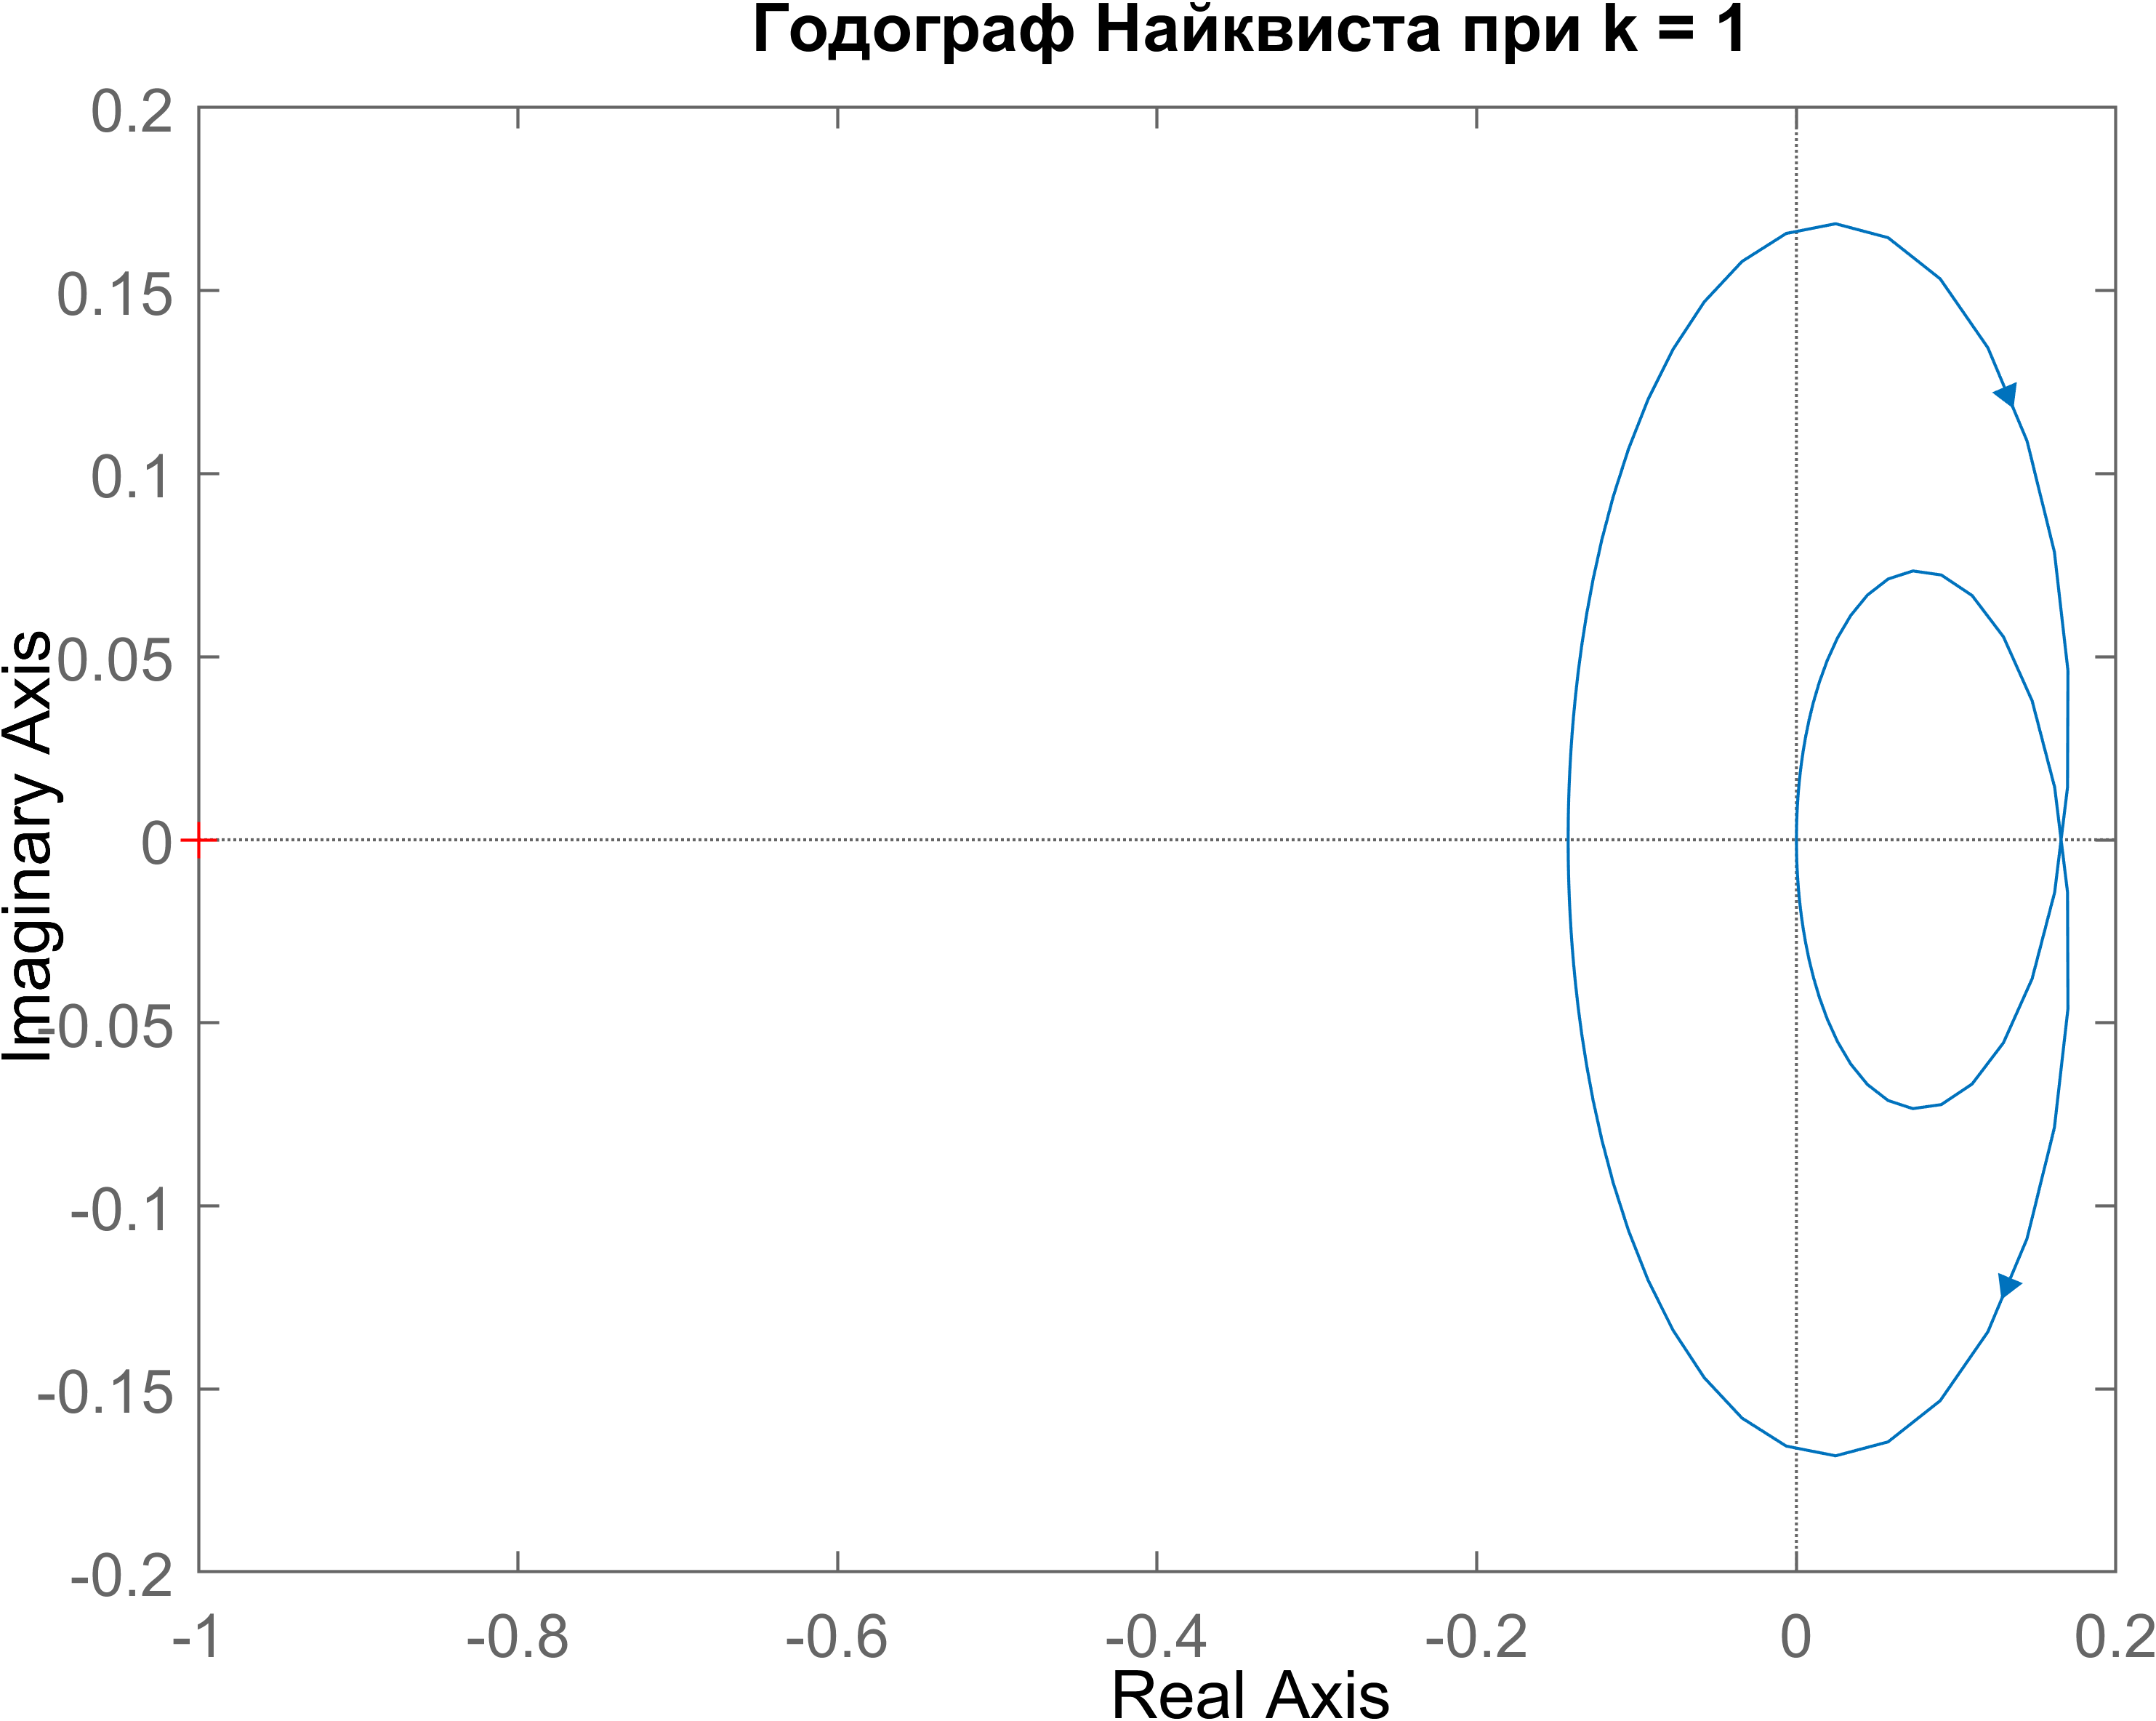
\includegraphics[width=0.7\textwidth, trim={0cm 0cm 0cm 0cm}]{../images/2_1_0_hod.png}
    \caption{Годограф Найквиста для $k = 1$}
\end{figure}

\begin{figure}[H]
    \centering
    \centering
    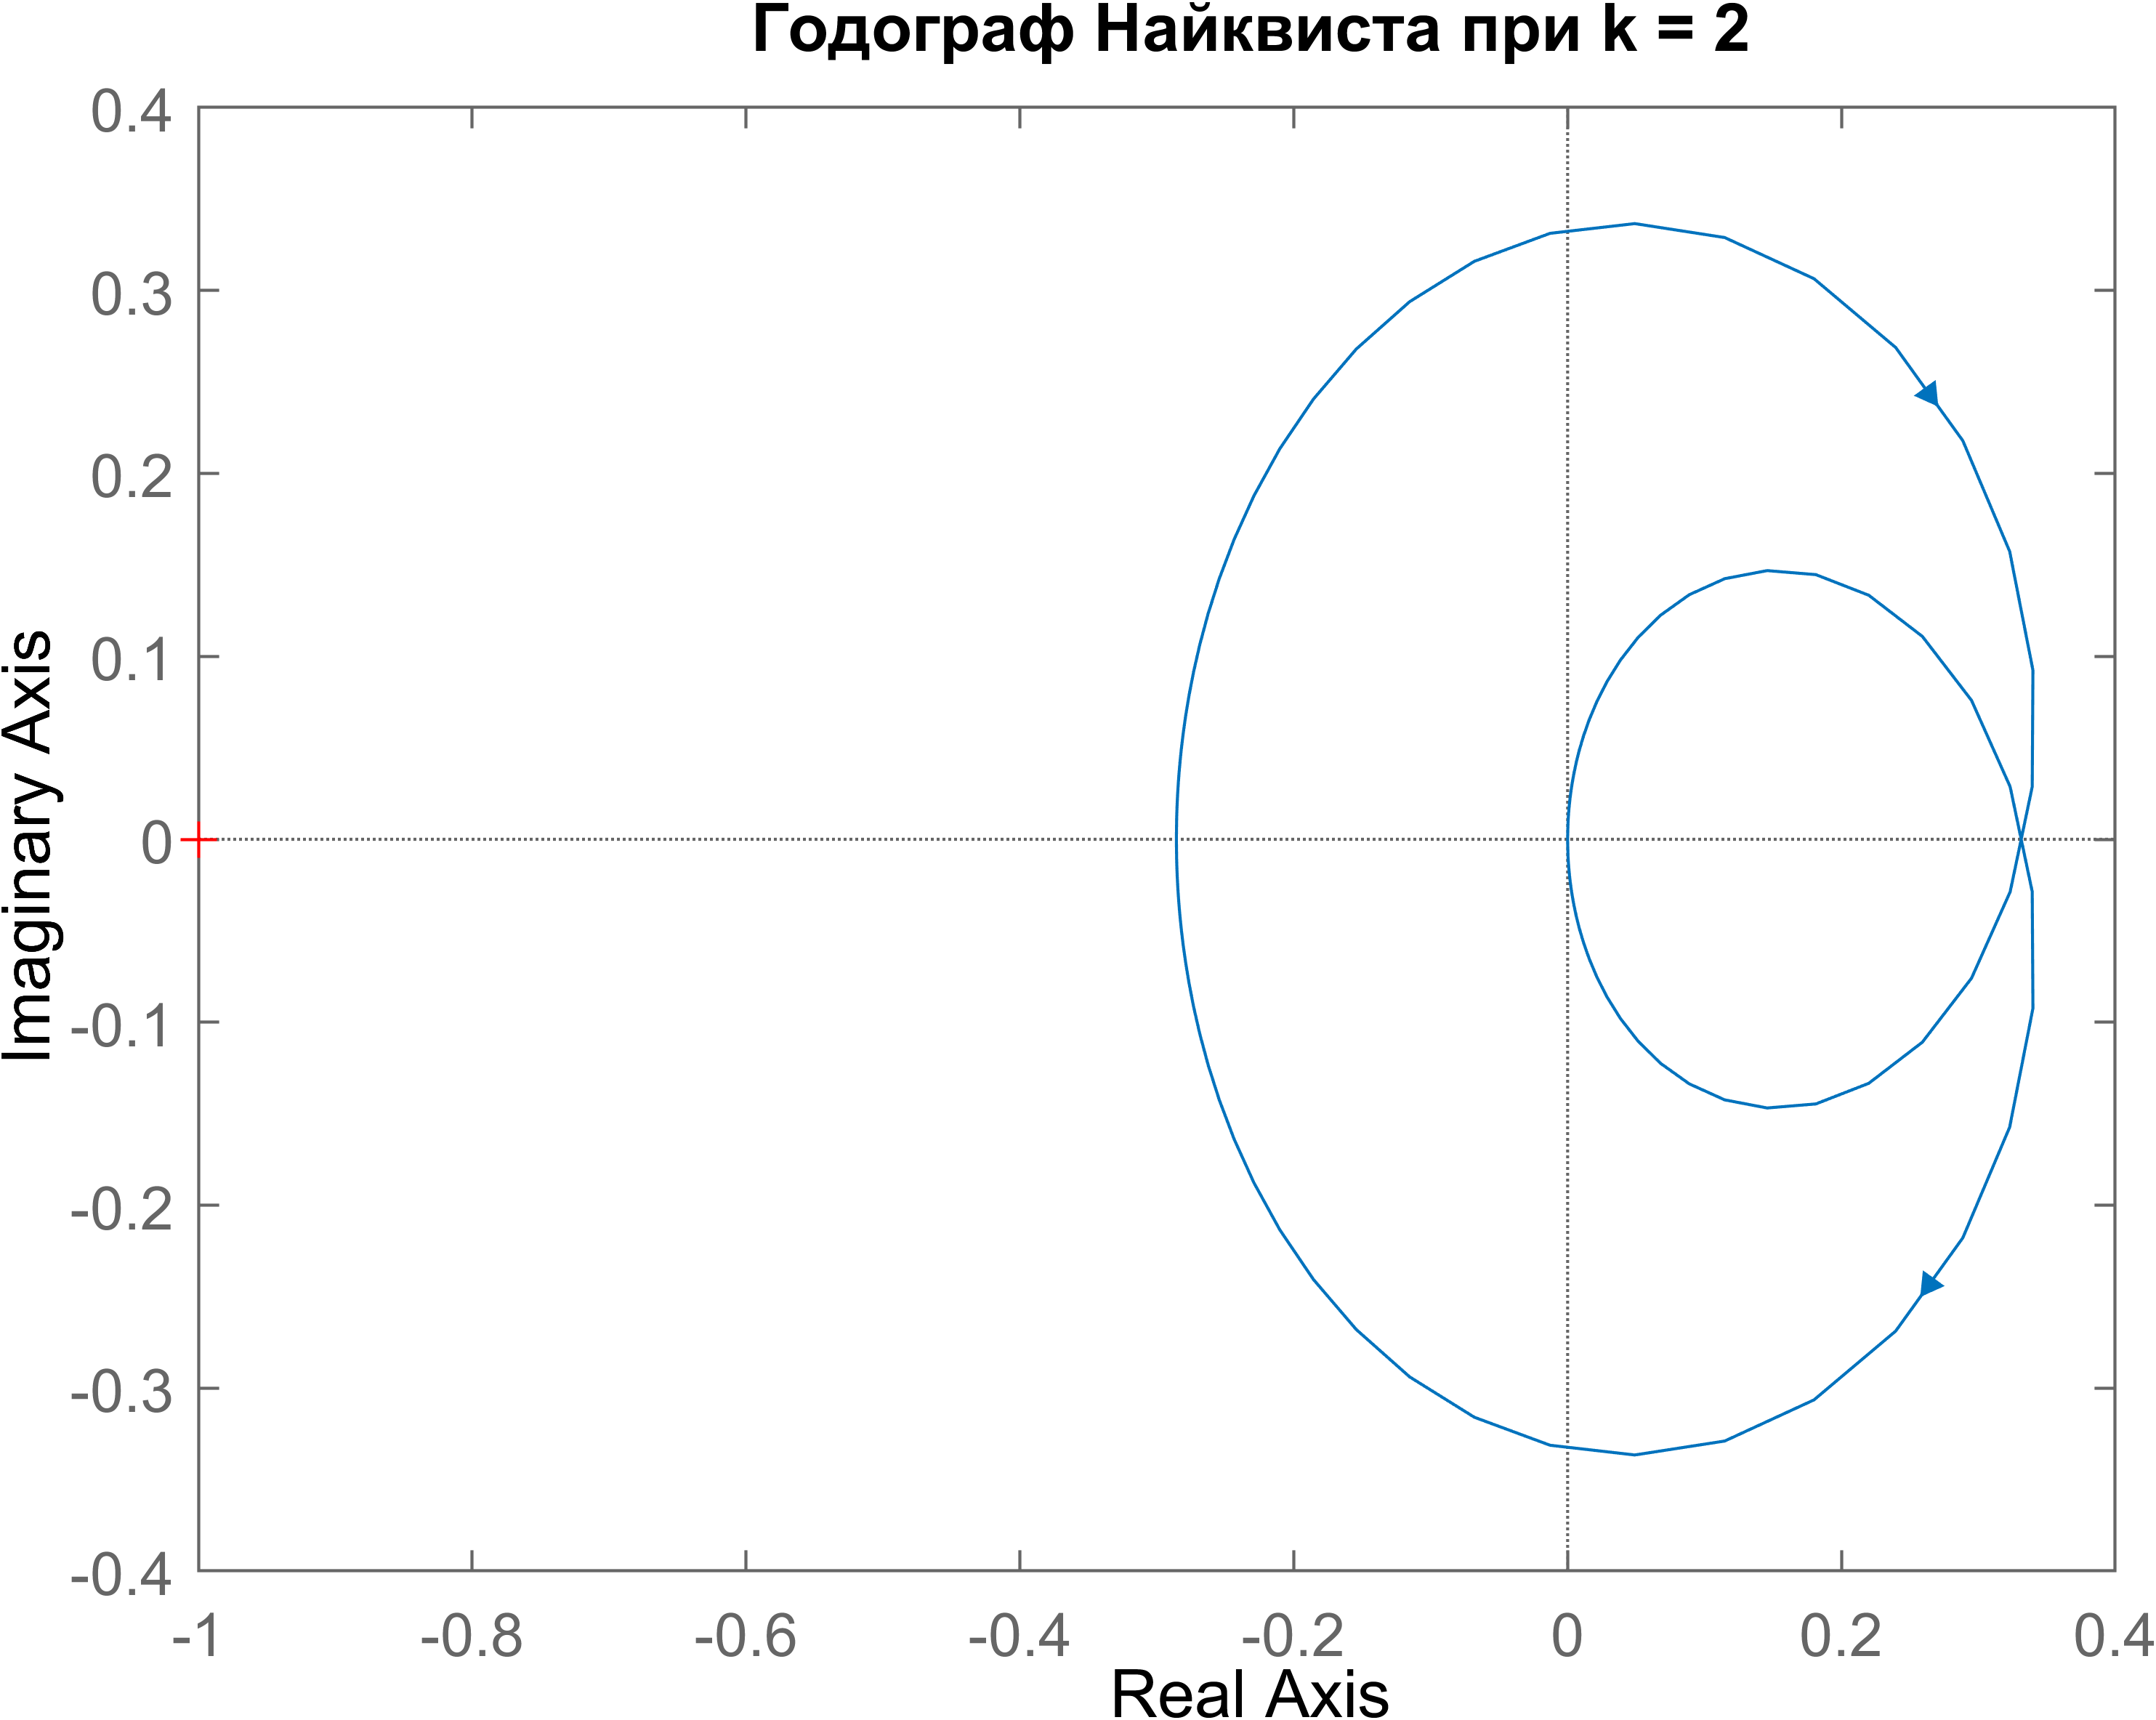
\includegraphics[width=0.7\textwidth, trim={0cm 0cm 0cm 0cm}]{../images/2_1_1_hod.png}
    \caption{Годограф Найквиста для $k = 2$}
\end{figure}

\begin{figure}[H]
    \centering
    \centering
    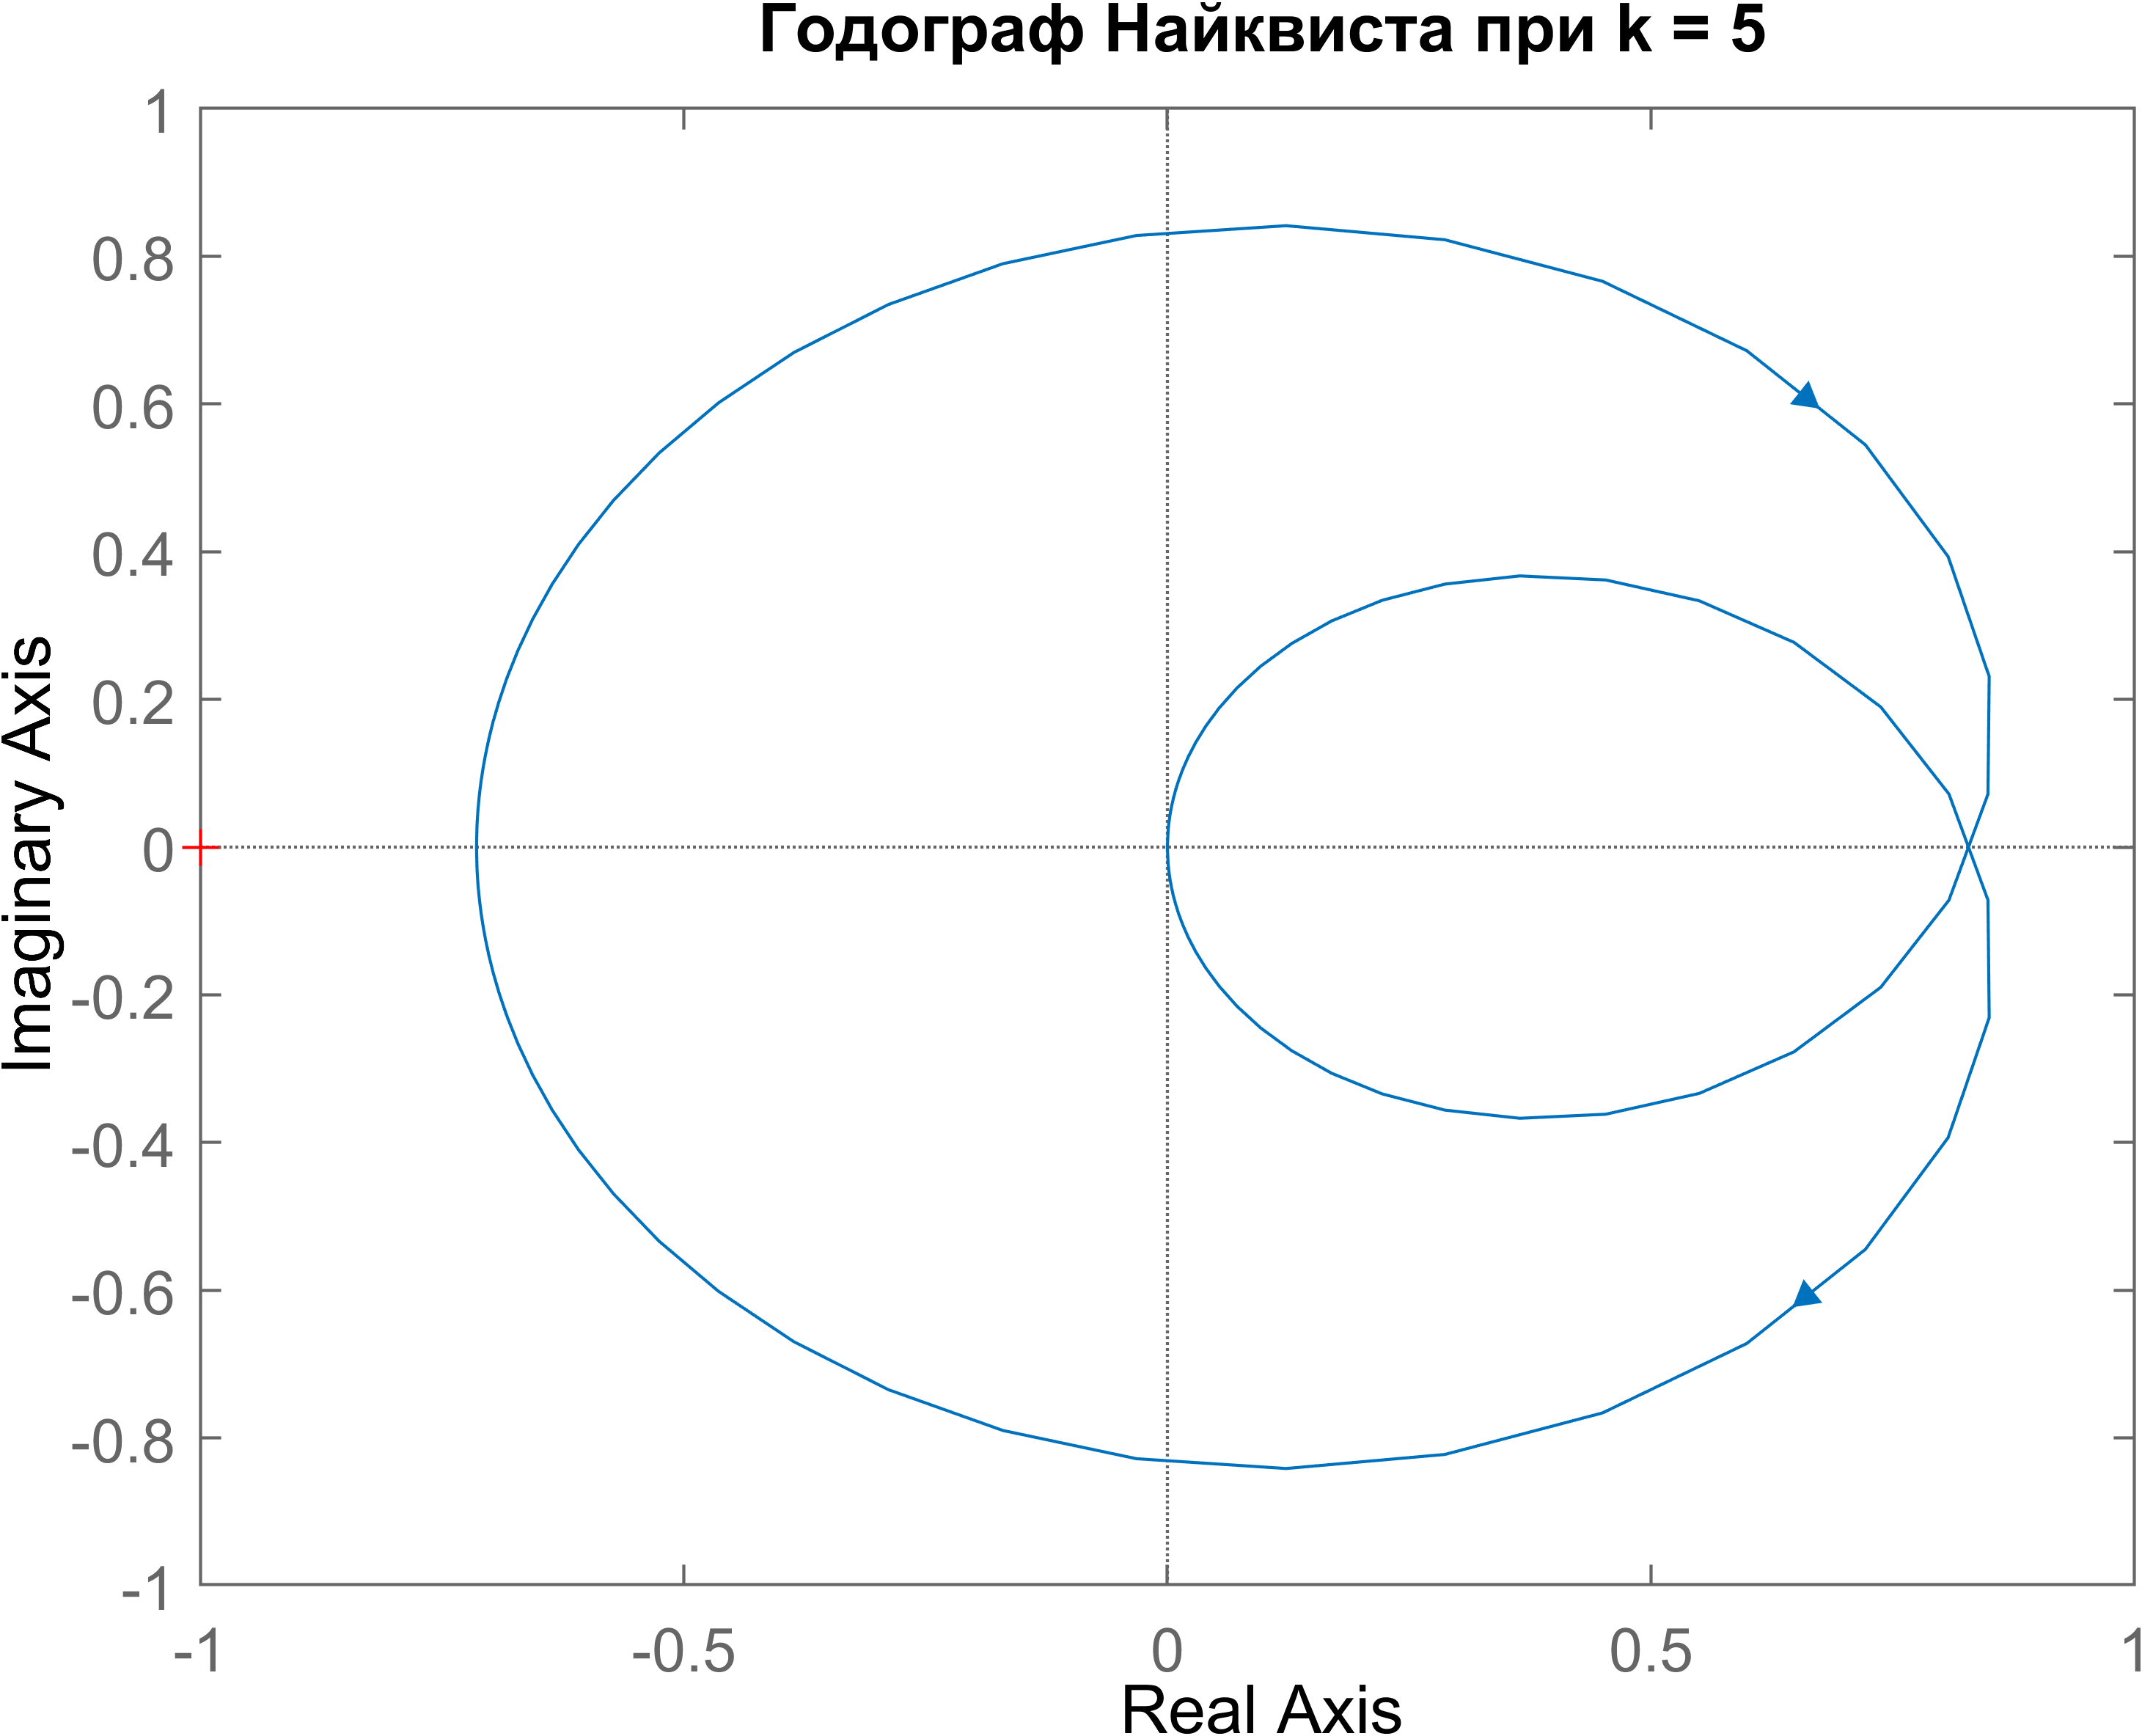
\includegraphics[width=0.7\textwidth, trim={0cm 0cm 0cm 0cm}]{../images/2_1_2_hod.png}
    \caption{Годограф Найквиста для $k = 5$}
\end{figure}

\begin{figure}[H]
    \centering
    \centering
    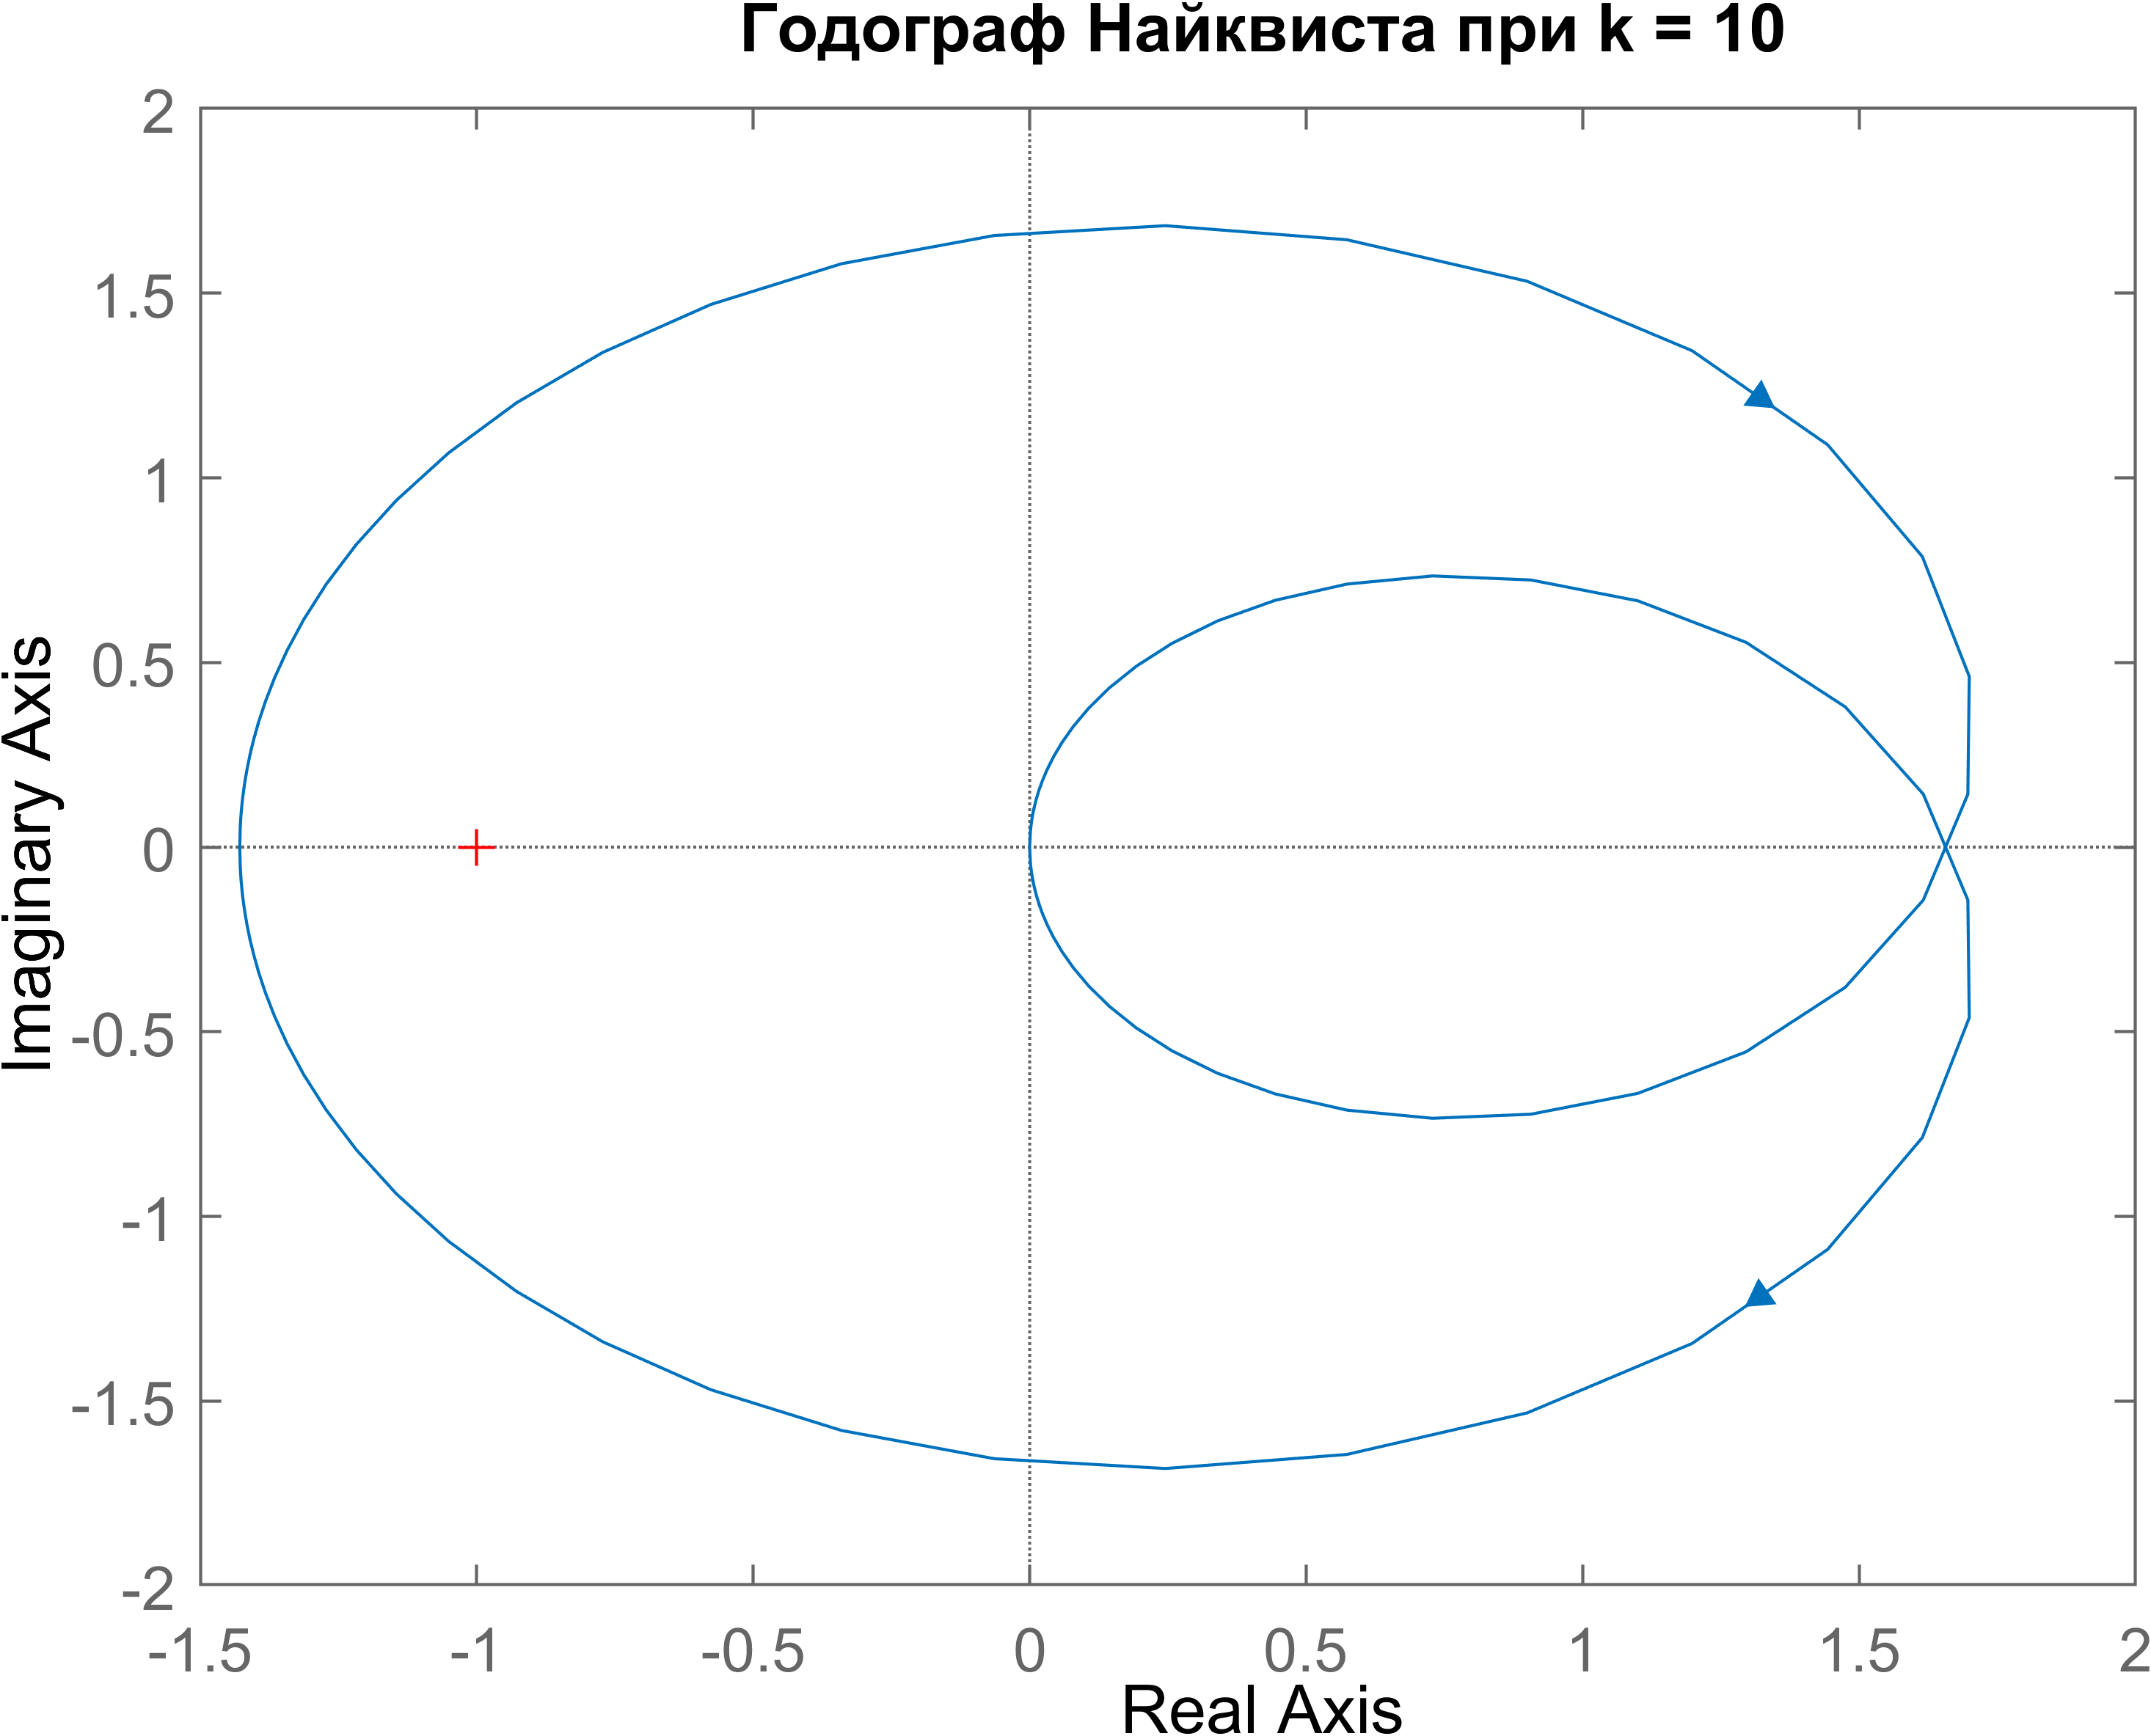
\includegraphics[width=0.7\textwidth, trim={0cm 0cm 0cm 0cm}]{../images/2_1_3_hod.png}
    \caption{Годограф Найквиста для $k = 10$}
\end{figure}

Как видим, при увеличении коэффициента усиления $k$ годограф увеличивается, в том числе в левой полуплоскости. 
С увеличением $k$ годограф начинает охватывать и точку $(-1, 0)$. Чтобы определить максимальное значение
коэффициента усиления, при котором система остается устойчивой, найдем аналитические выражения для 
частотных характеристик системы:
\[
W_1(j\omega) = \frac{k(j\omega - 1)}{-\omega^2 + 6j\omega + 7} = \frac{-\omega^3i + 7\omega^2 +13\omega i - 7}{\omega^4 + 22\omega^2 + 49}
\]
\[
A_1(\omega) = \frac{\sqrt{\omega^2+1}}{\sqrt{\omega^4 + 22\omega^2 + 49}}
\]
\[
\varphi_1(\omega) = atan2\left(\frac{-\omega^3 + 13\omega}{\omega^4 + 22\omega^2 + 49},\frac{7\omega^2 - 7}{\omega^4 + 22\omega^2 + 49}\right)
\]

Теперь найдем значение критической частоты и с помощью нее найдем максимальное значение коэффициента усиления:
\[
\varphi_1(\omega_{\text{кр}}) = -\pi \Rightarrow \omega_{\text{кр}} = 0
\]
\[
k_{\text{макс}} = \frac{1}{A_1(\omega_{\text{кр}})} = 7
\]

Продемонстрируем переходные характеристики системы при коэффициентах k, соответствующих устойчивости и неустойчивости:
\begin{figure}[H]
    \centering
    \begin{minipage}{0.45\textwidth}
        \centering
        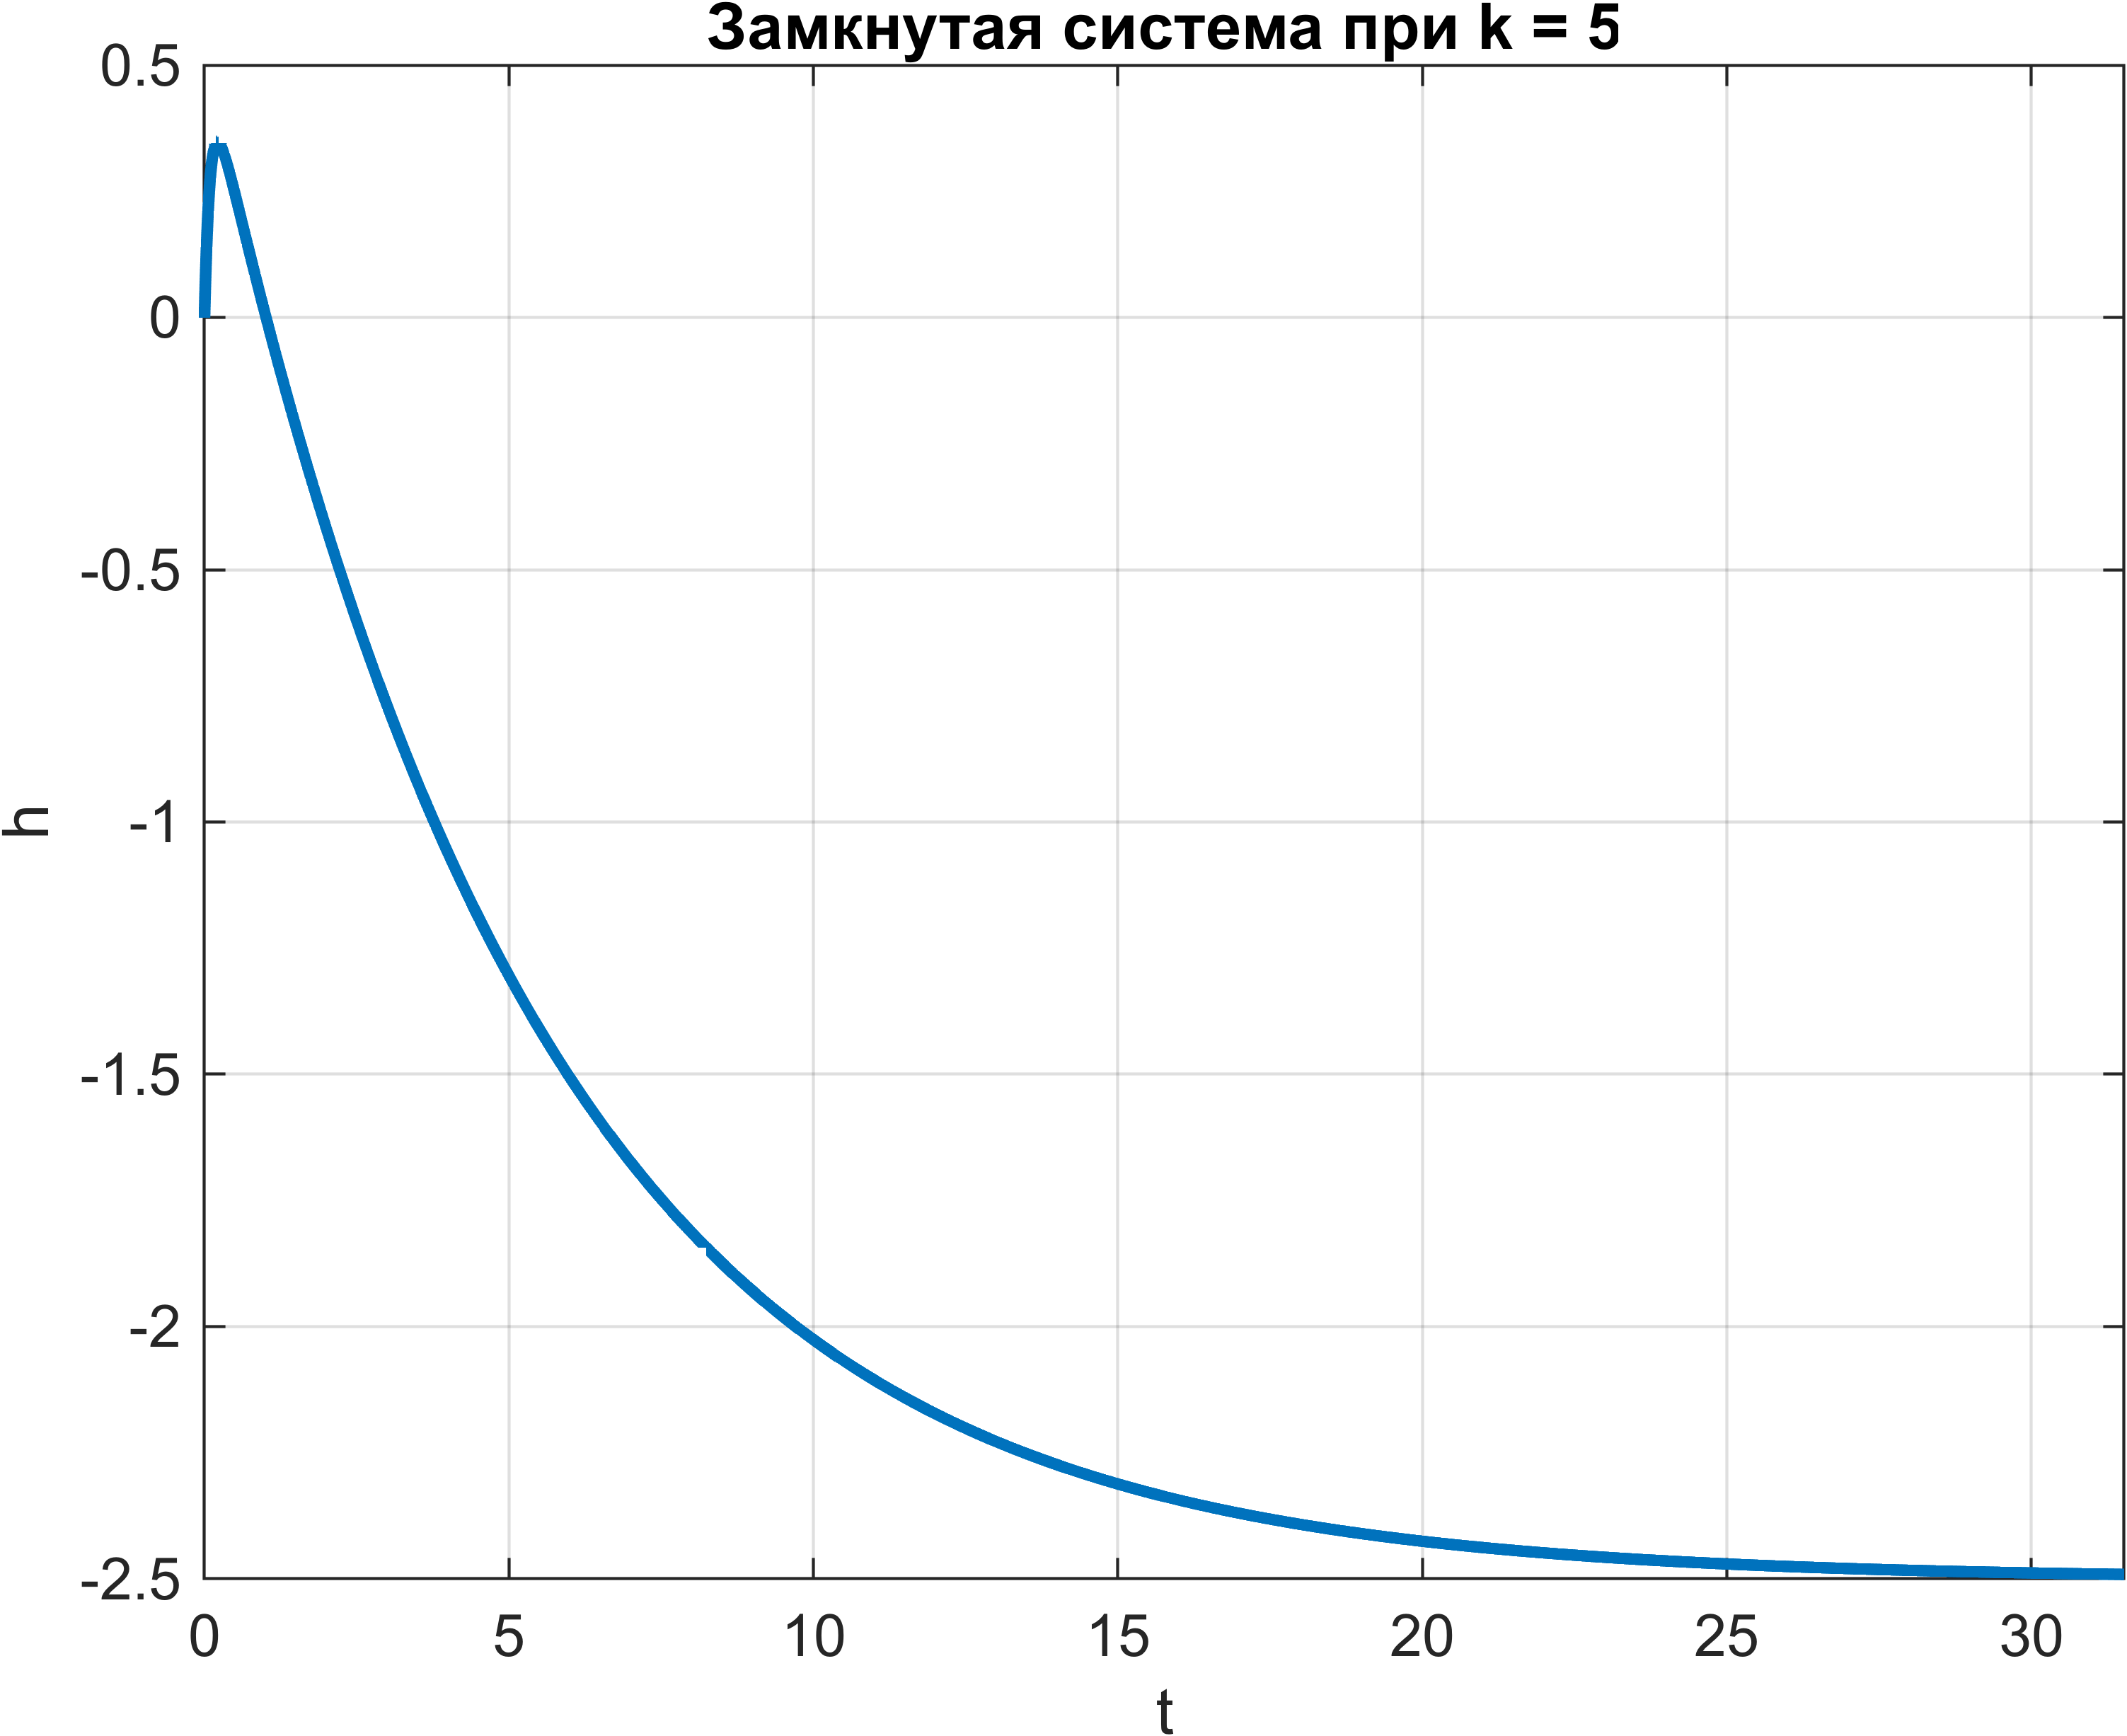
\includegraphics[width=1\textwidth, trim={0cm 0cm 0cm 0cm}]{../images/2_1_1_cl.png}
    \end{minipage}
    \hfill
    \begin{minipage}{0.45\textwidth}
        \centering
        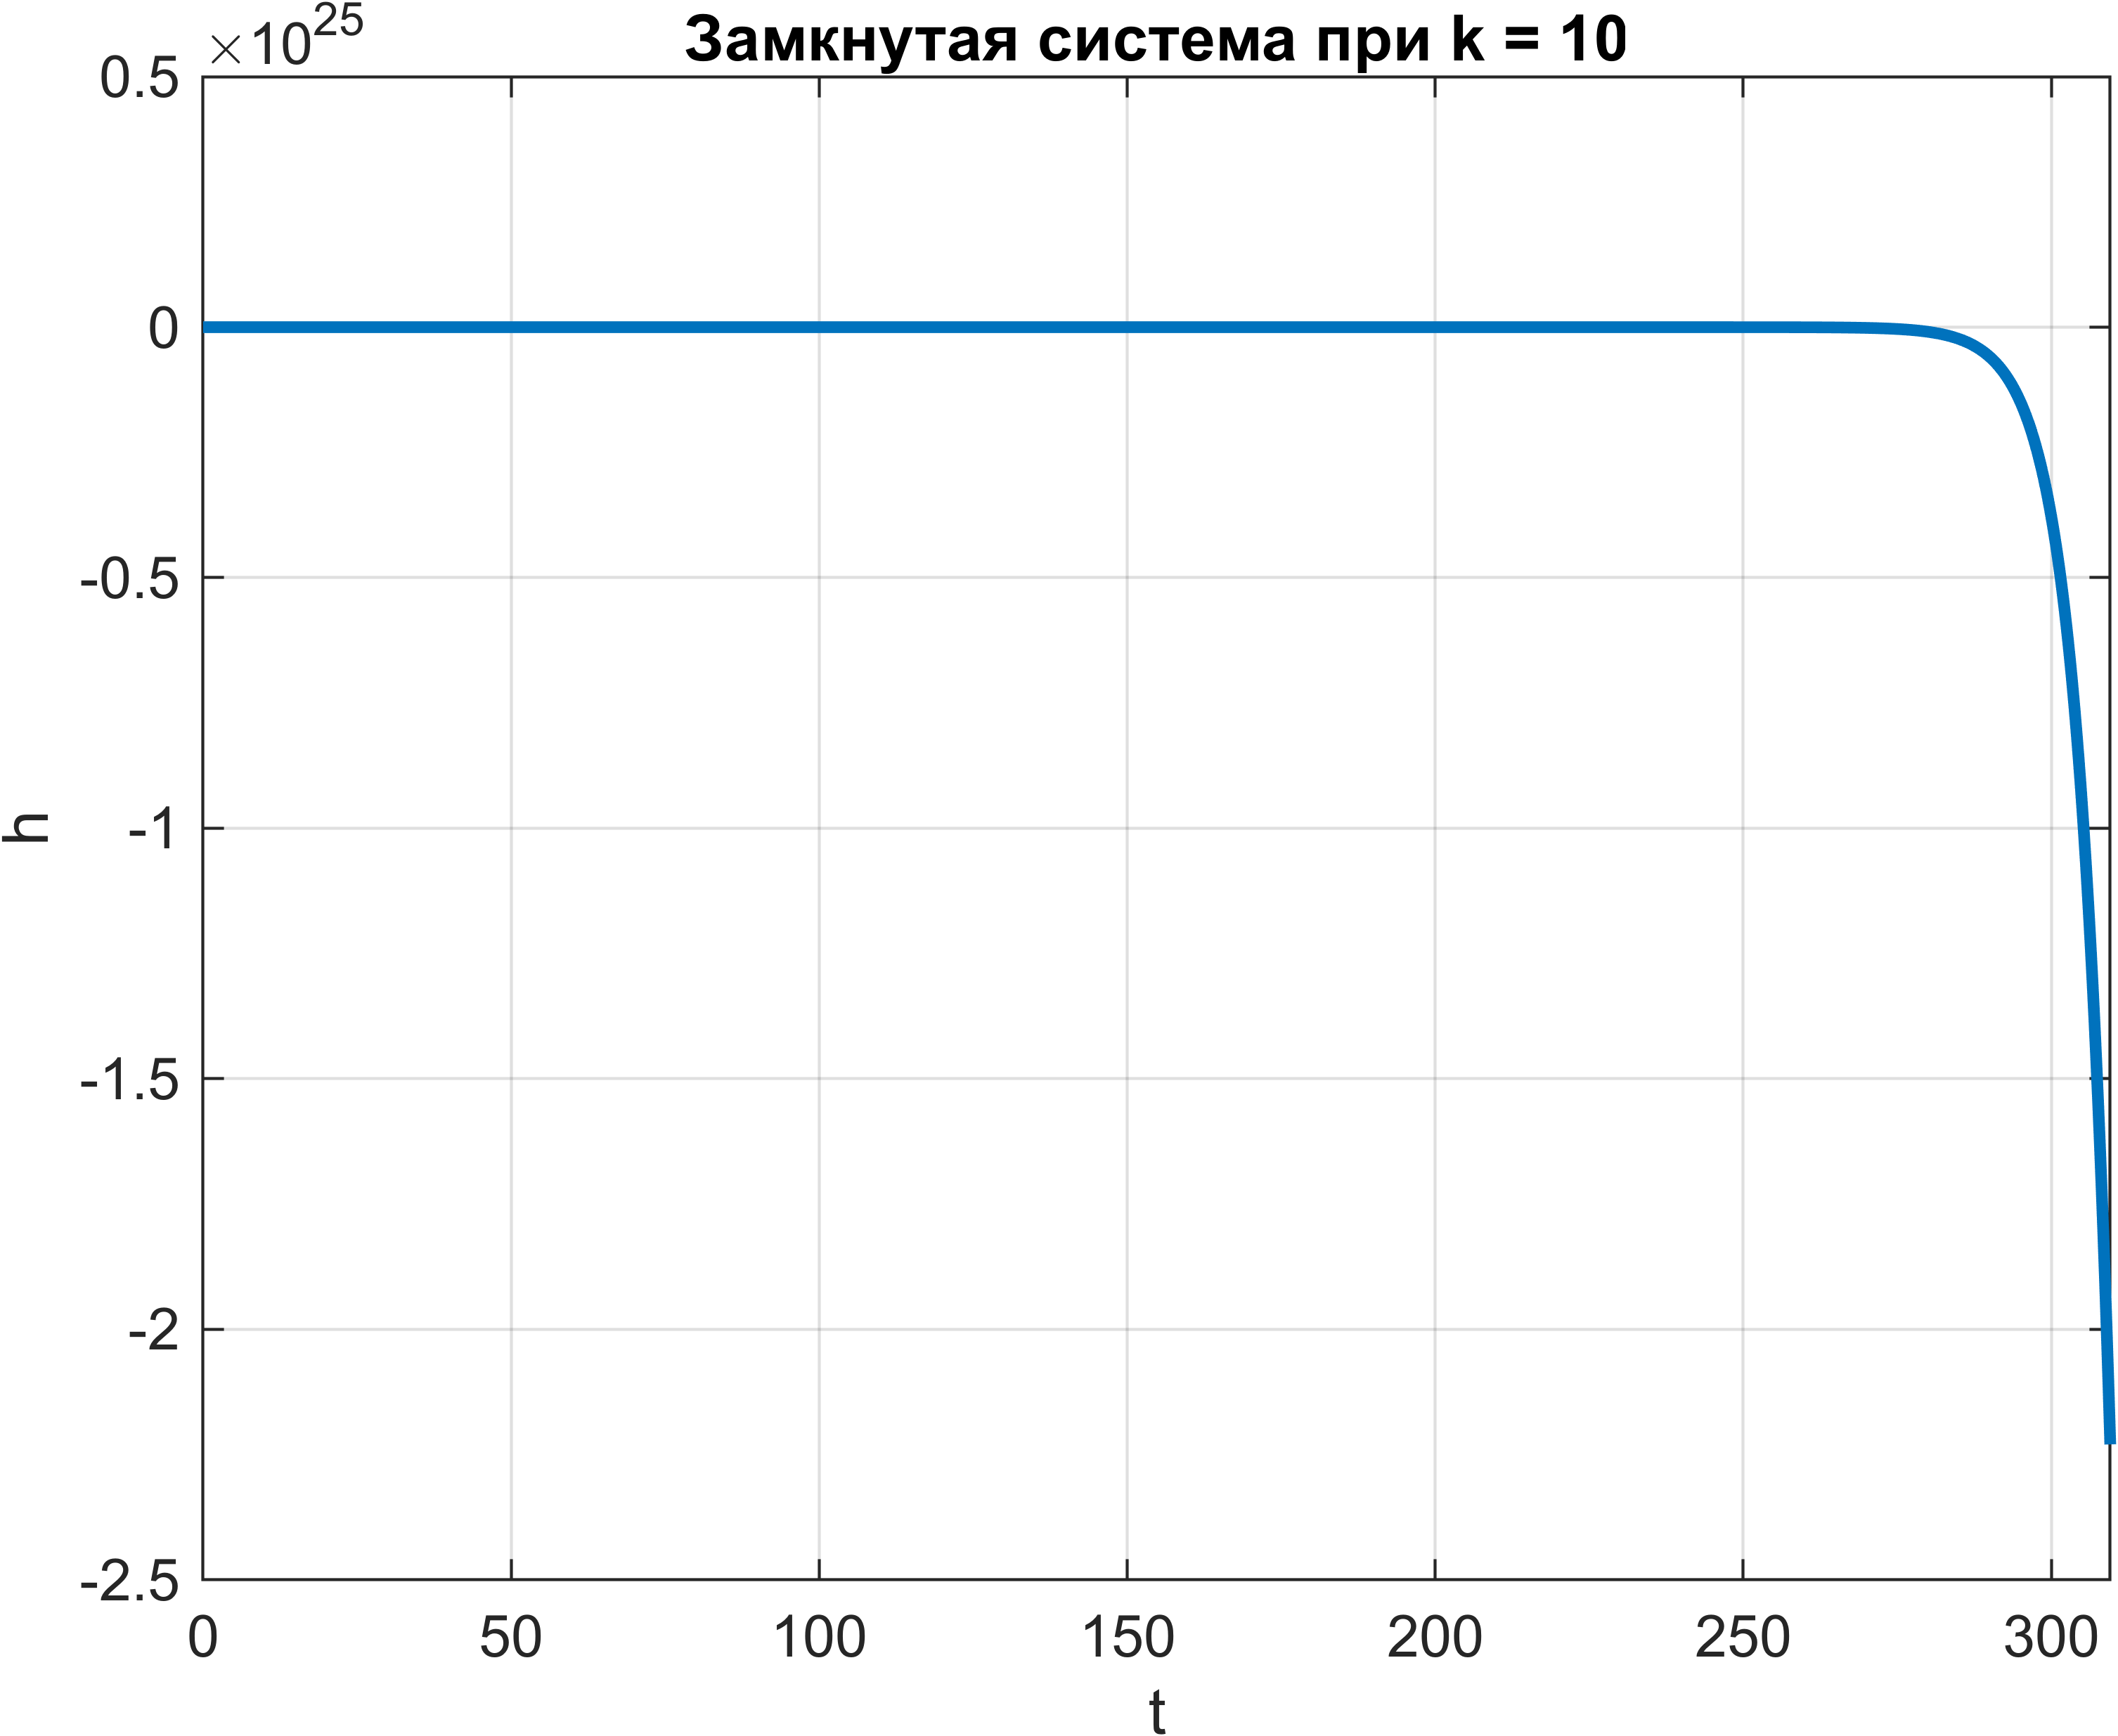
\includegraphics[width=1\textwidth, trim={0cm 0cm 0cm 0cm}]{../images/2_1_2_cl.png}
    \end{minipage}
    \caption{Переходные характеристики системы при $k = 5$ и $k = 10$}
\end{figure}

\section{Передаточная функция $W_2(s)$}
Построим годограф Найквиста для передаточных функций с различными значениями коэффициента усиления $k$:
\begin{enumerate}
    \item $k = 1$:
    \item $k = 0.3$:
    \item $k = 2$:
    \item $k = 5$:
\end{enumerate}

\begin{figure}[H]
    \centering
    \centering
    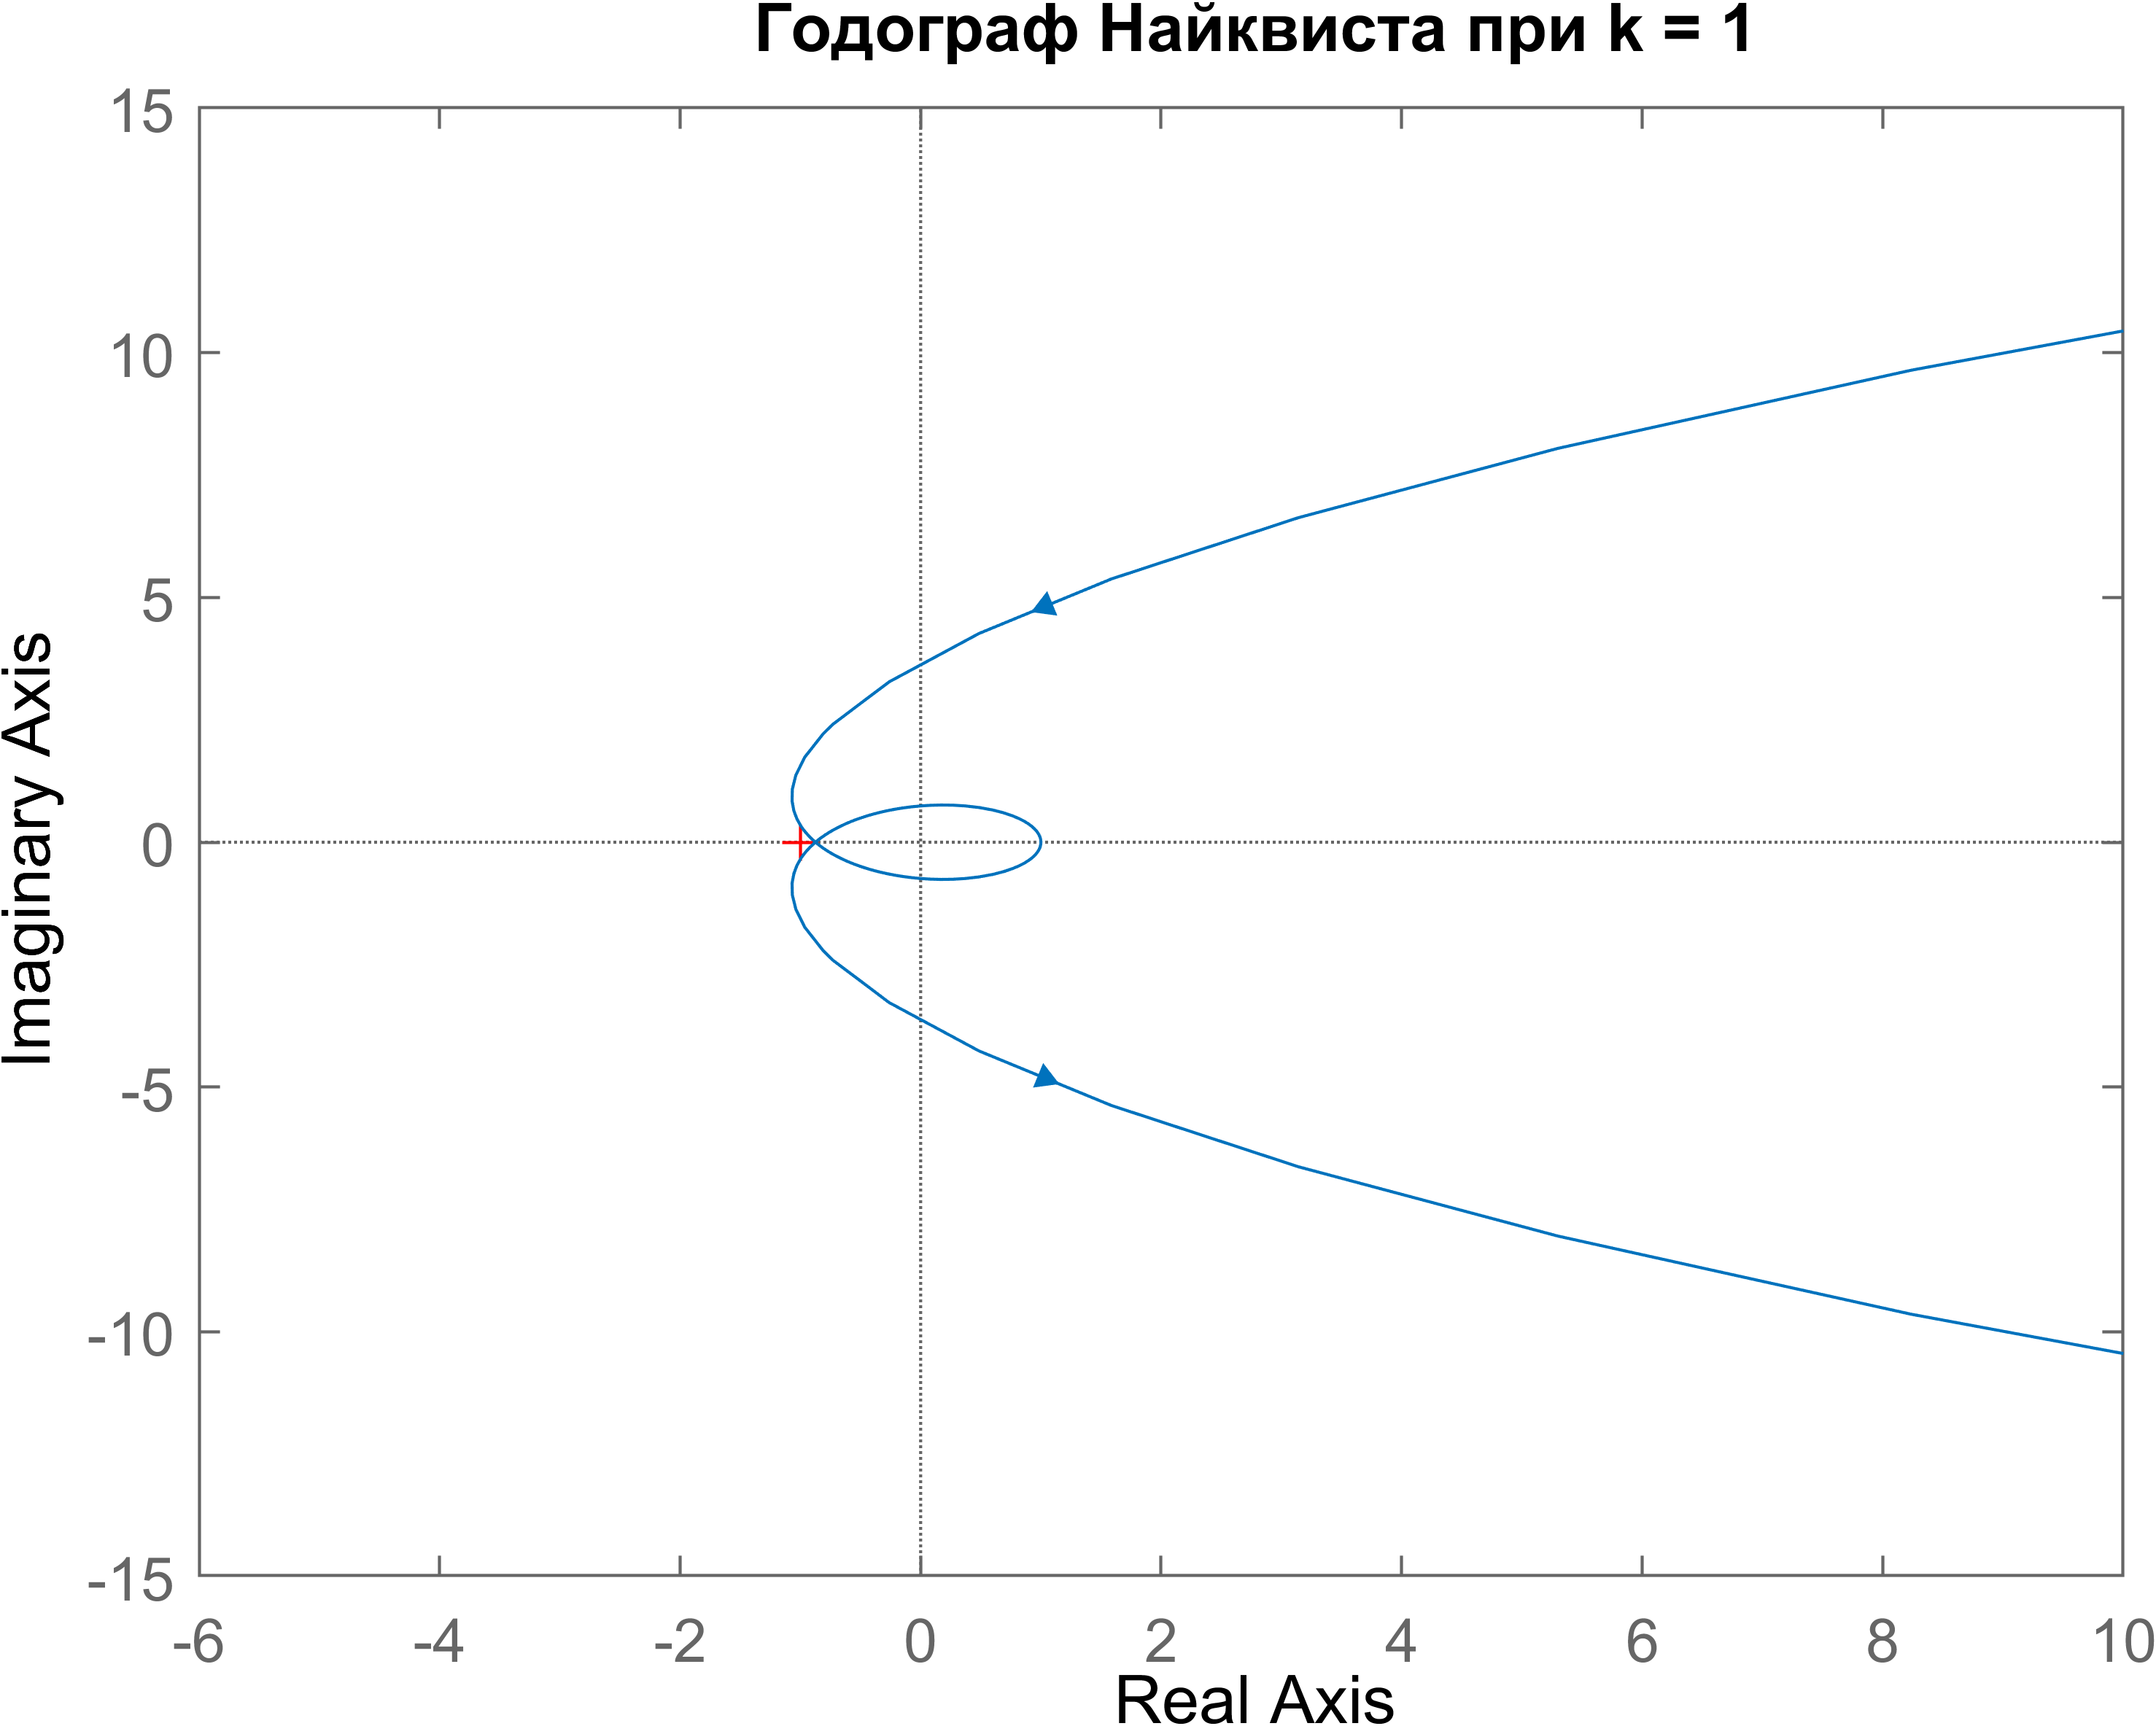
\includegraphics[width=0.7\textwidth, trim={0cm 0cm 0cm 0cm}]{../images/2_2_0_hod.png}
    \caption{Годограф Найквиста для $k = 1$}
\end{figure}

\begin{figure}[H]
    \centering
    \centering
    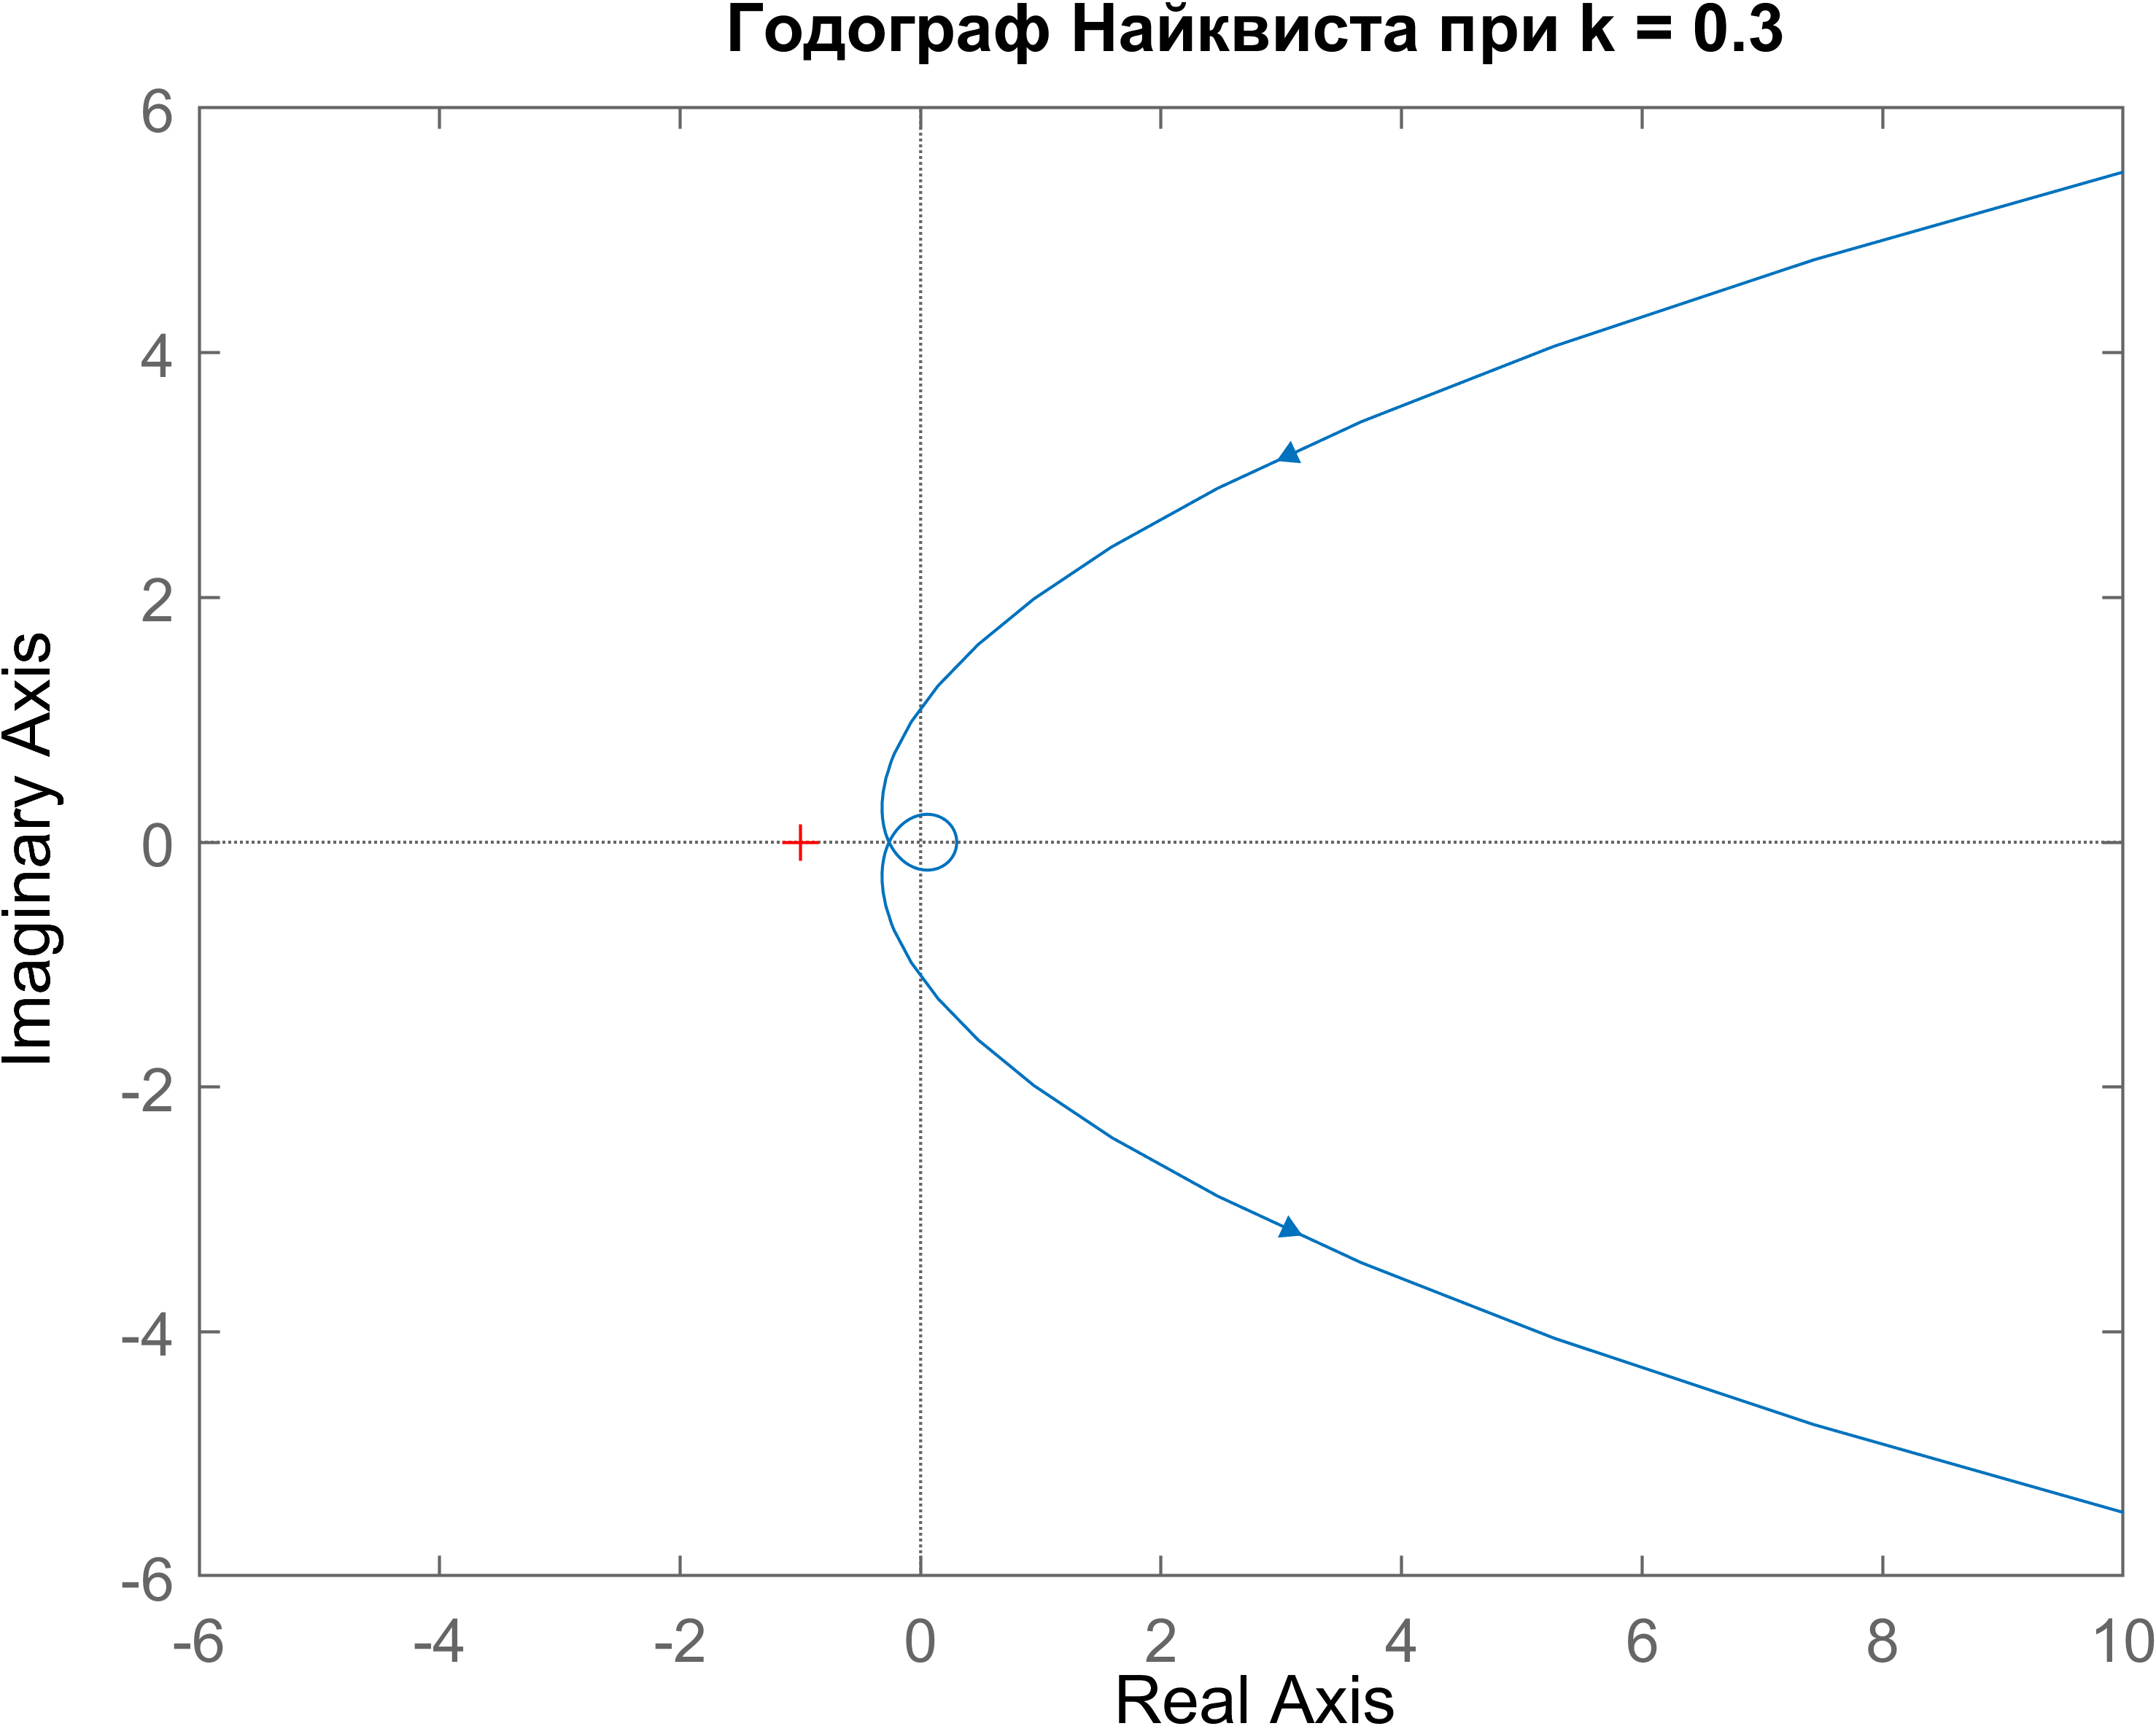
\includegraphics[width=0.7\textwidth, trim={0cm 0cm 0cm 0cm}]{../images/2_2_1_hod.png}
    \caption{Годограф Найквиста для $k = 0.3$}
\end{figure}

\begin{figure}[H]
    \centering
    \centering
    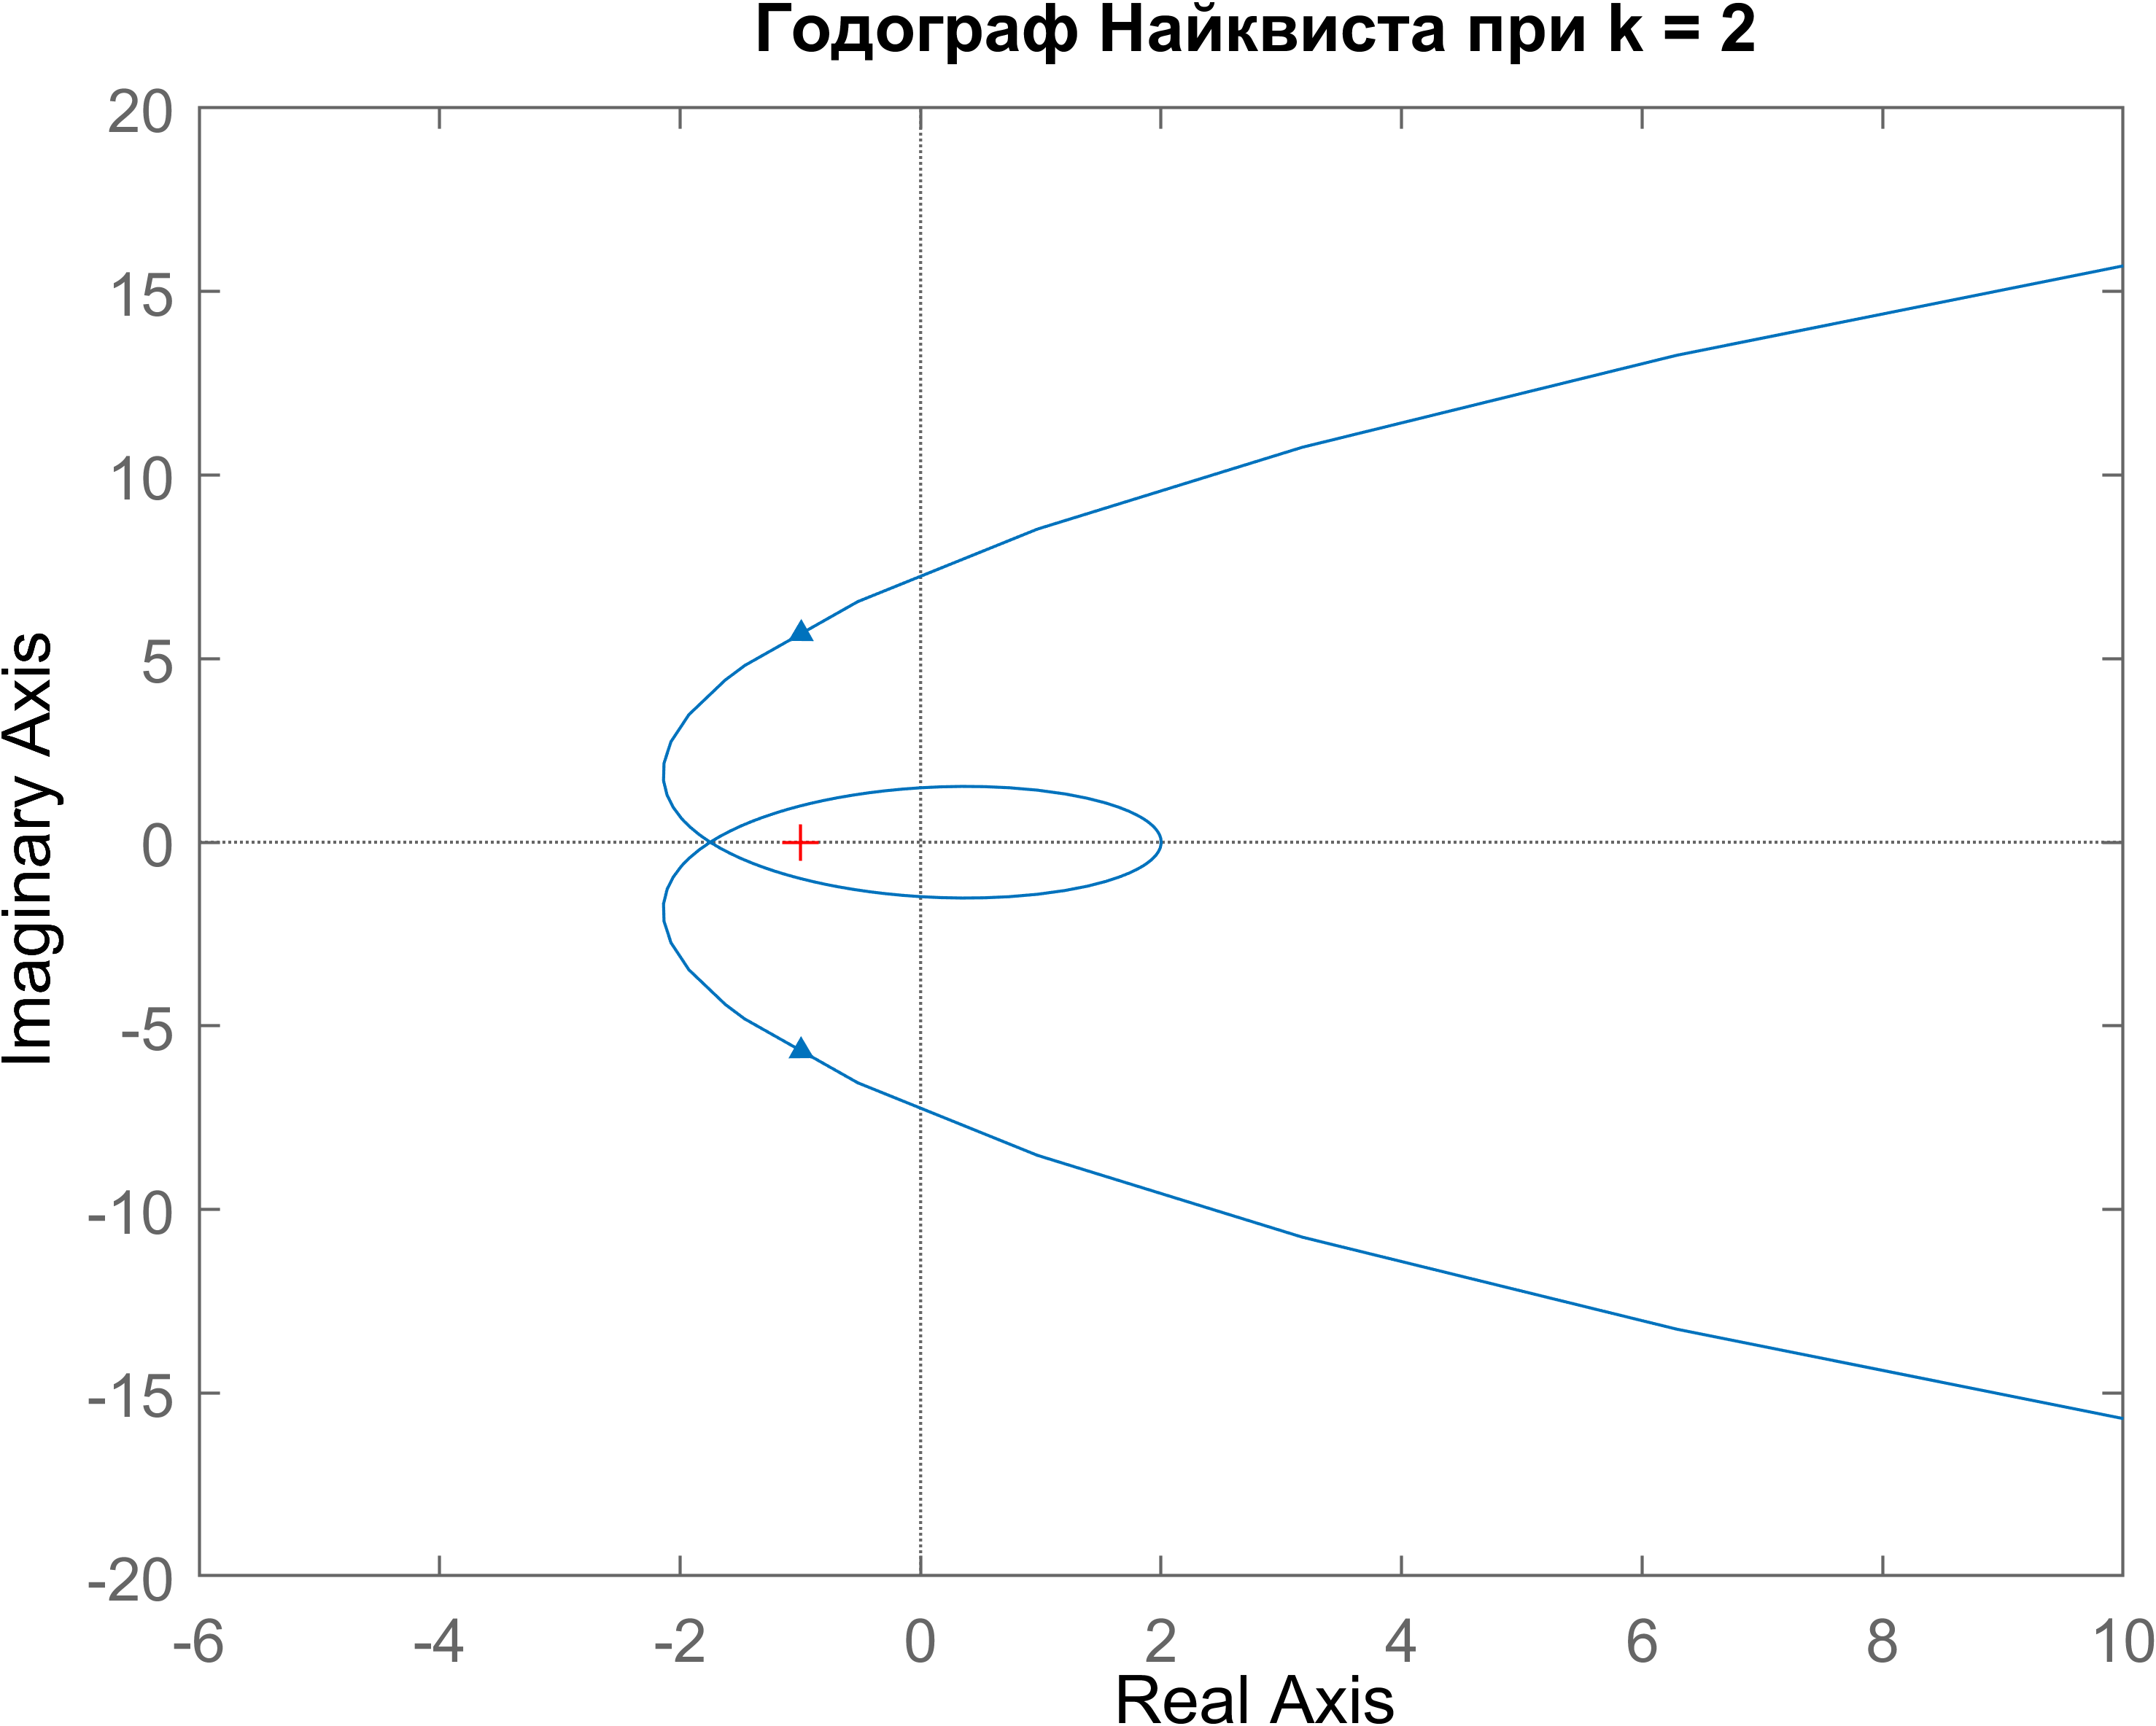
\includegraphics[width=0.7\textwidth, trim={0cm 0cm 0cm 0cm}]{../images/2_2_2_hod.png}
    \caption{Годограф Найквиста для $k = 2$}
\end{figure}

\begin{figure}[H]
    \centering
    \centering
    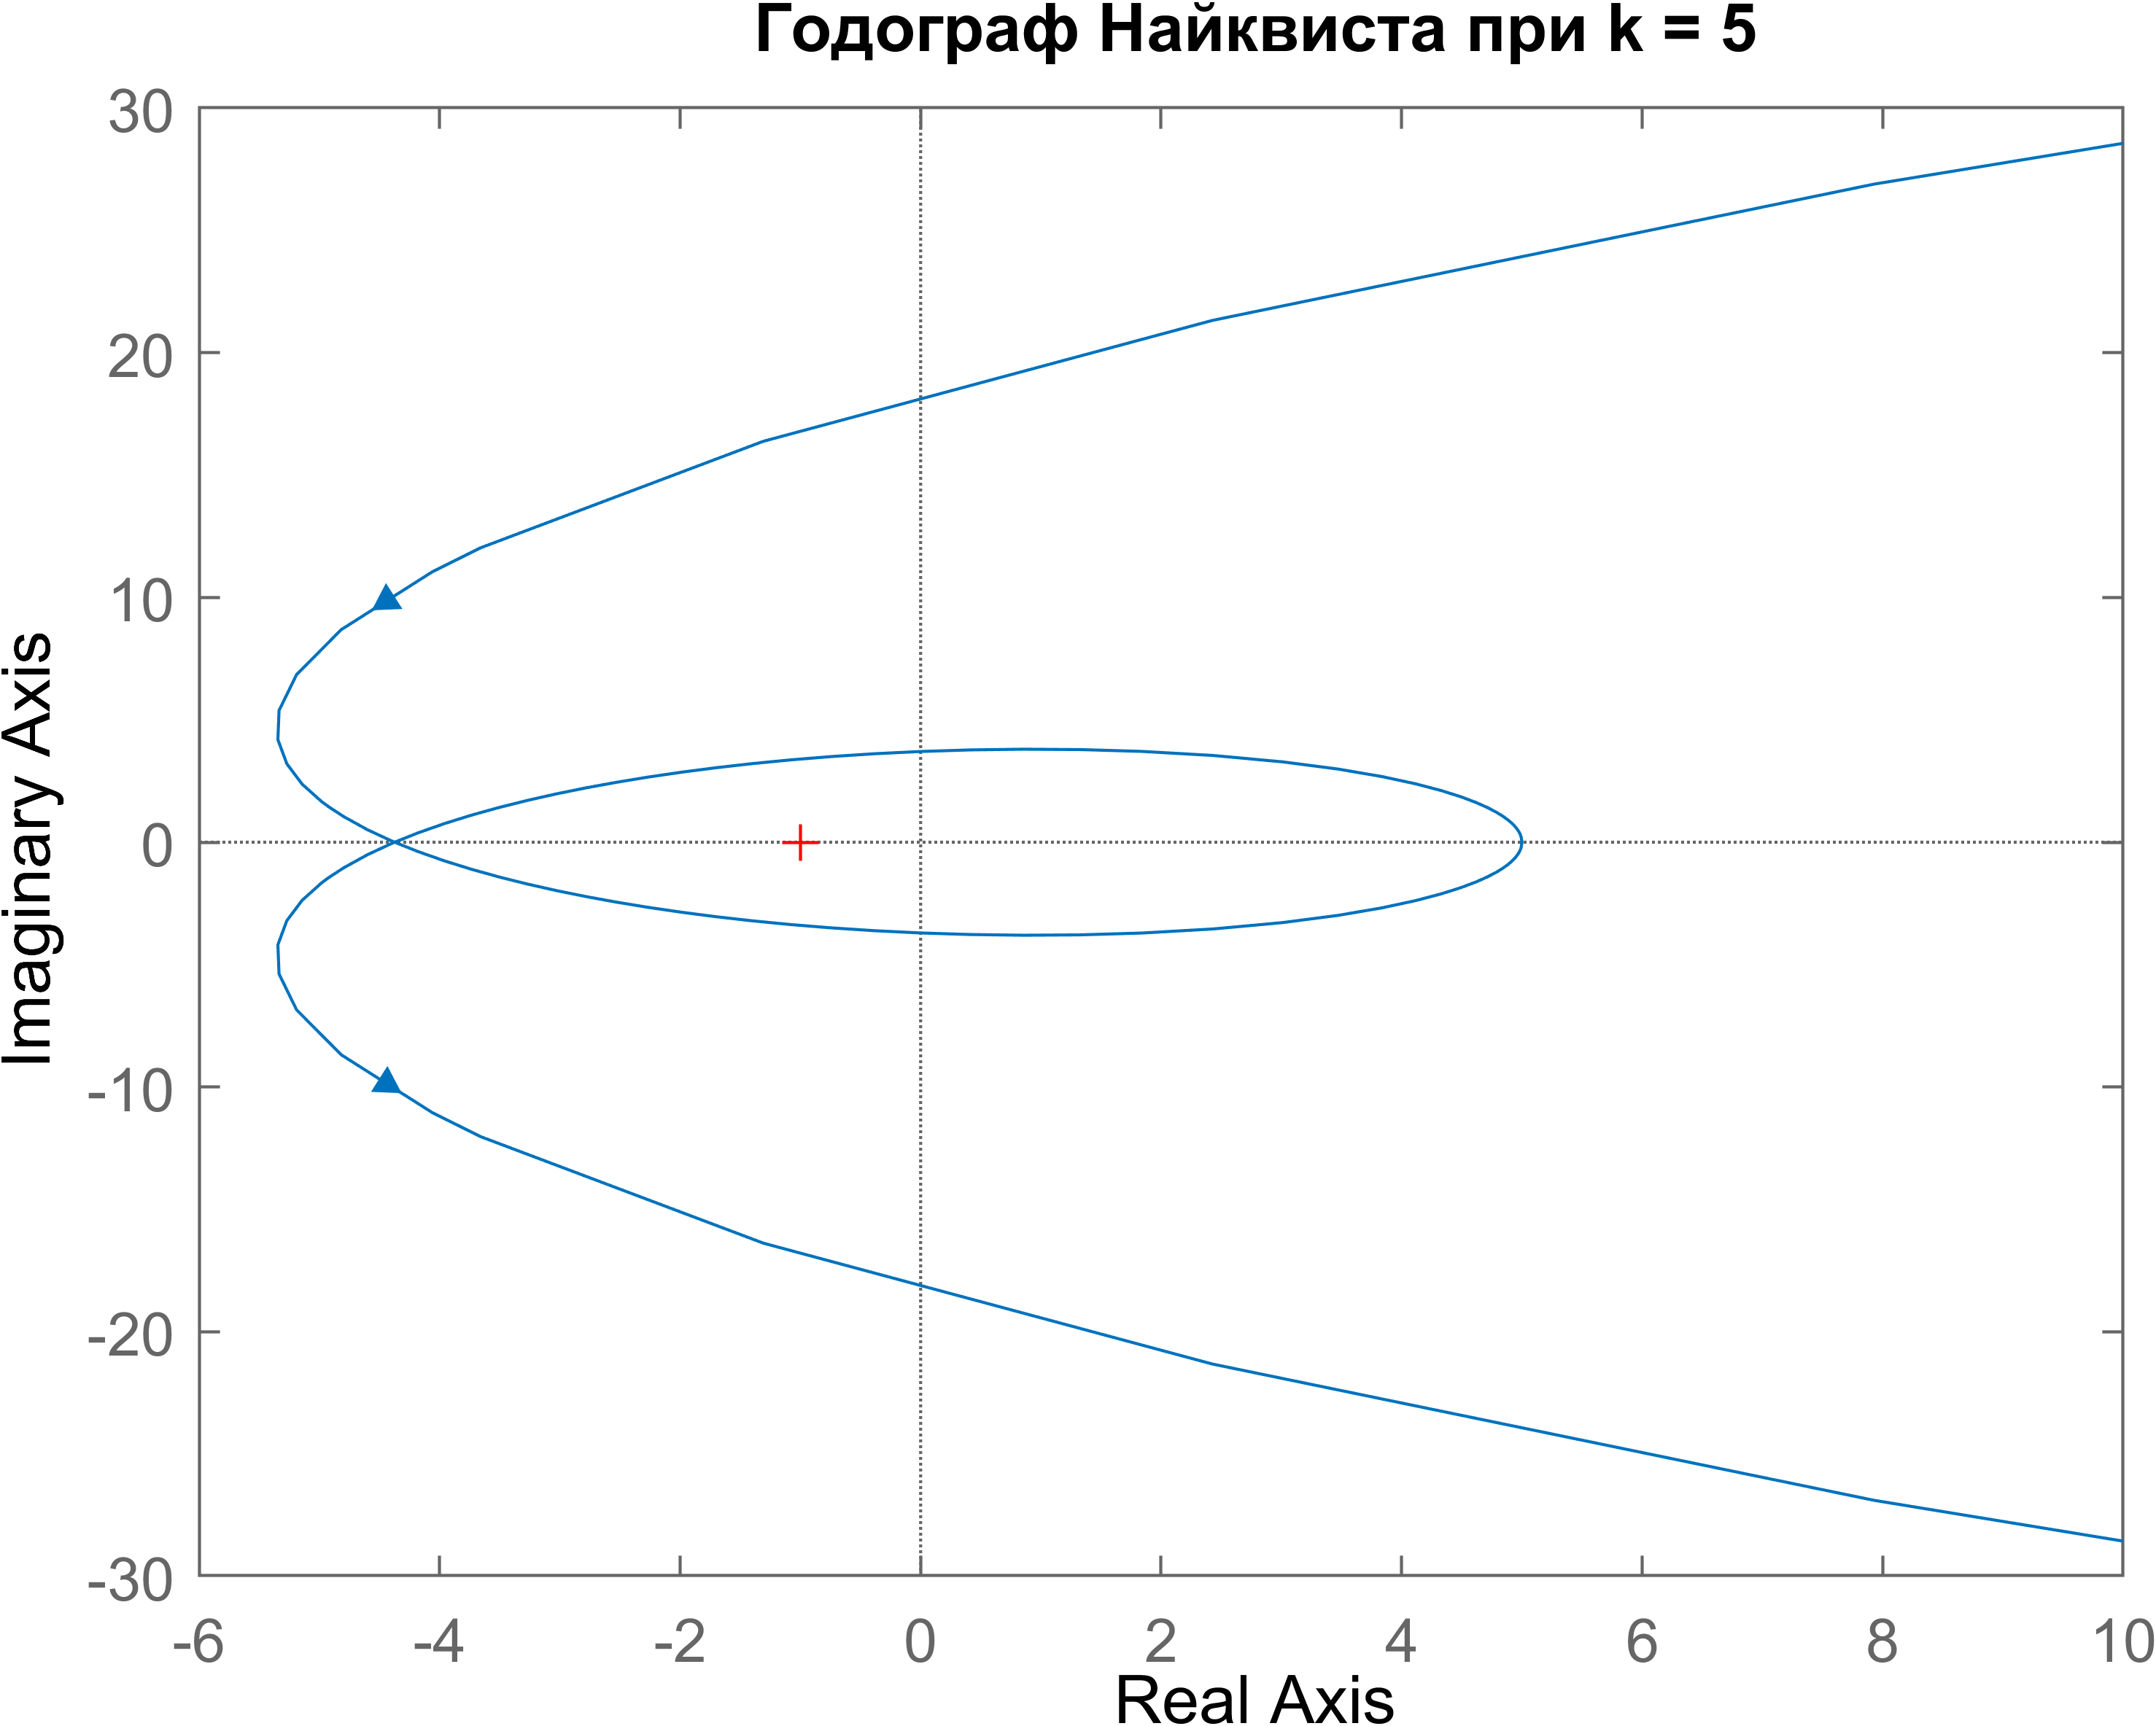
\includegraphics[width=0.7\textwidth, trim={0cm 0cm 0cm 0cm}]{../images/2_2_3_hod.png}
    \caption{Годограф Найквиста для $k = 5$}
\end{figure}

Как видим, годограф не замкнут, но имеет "петлю" в левой полуплоскости. При увеличении коэффициента усиления $k$ петля увеличивается
и петля охватывает точку $(-1, 0)$. Система устойчива только если петля охватывает точку $(-1, 0)$. Найдем миниальное
значение коэффициента усиления, при котором система остается устойчивой:
\[
W_2(j\omega) = \frac{-\omega ^3 10j - 15\omega ^2 + \omega 18j + 6}{10\omega ^2 - \omega ^3 10j} =
\]
\[
= \frac{100\omega ^6 - \omega ^5 250j - 330\omega ^4 + \omega ^3 240j + 60\omega ^2}{100\omega ^6 + 100\omega ^4}
\]
\[
A_2(\omega) = \frac{\sqrt{100\omega ^6 - 135\omega ^4 + 144\omega ^2 + 36}}{10\omega ^2 \sqrt{\omega ^2 + 1}}
\]
\[
\varphi_2(\omega) = \mathrm{atan2}\left(\frac{240\omega ^3 - 250\omega ^5}{100\omega ^6 + 100\omega ^4}, \frac{100\omega ^6 - 330\omega ^4 + 60\omega ^2}{100\omega ^6 + 100\omega ^4}\right)
\]
\[
\varphi_1(\omega_{\text{кр}}) = -\pi \Rightarrow \omega_{\text{кр}} = \frac{-2\sqrt{6}}{5}
\]
\[
k_{\text{мин}} = \frac{1}{A_1(\omega_{\text{кр}})} = \frac{8}{7}
\]

Продемонстрируем переходные характеристики системы при коэффициентах k, соответствующих устойчивости и неустойчивости:
\begin{figure}[H]
    \centering
    \begin{minipage}{0.45\textwidth}
        \centering
        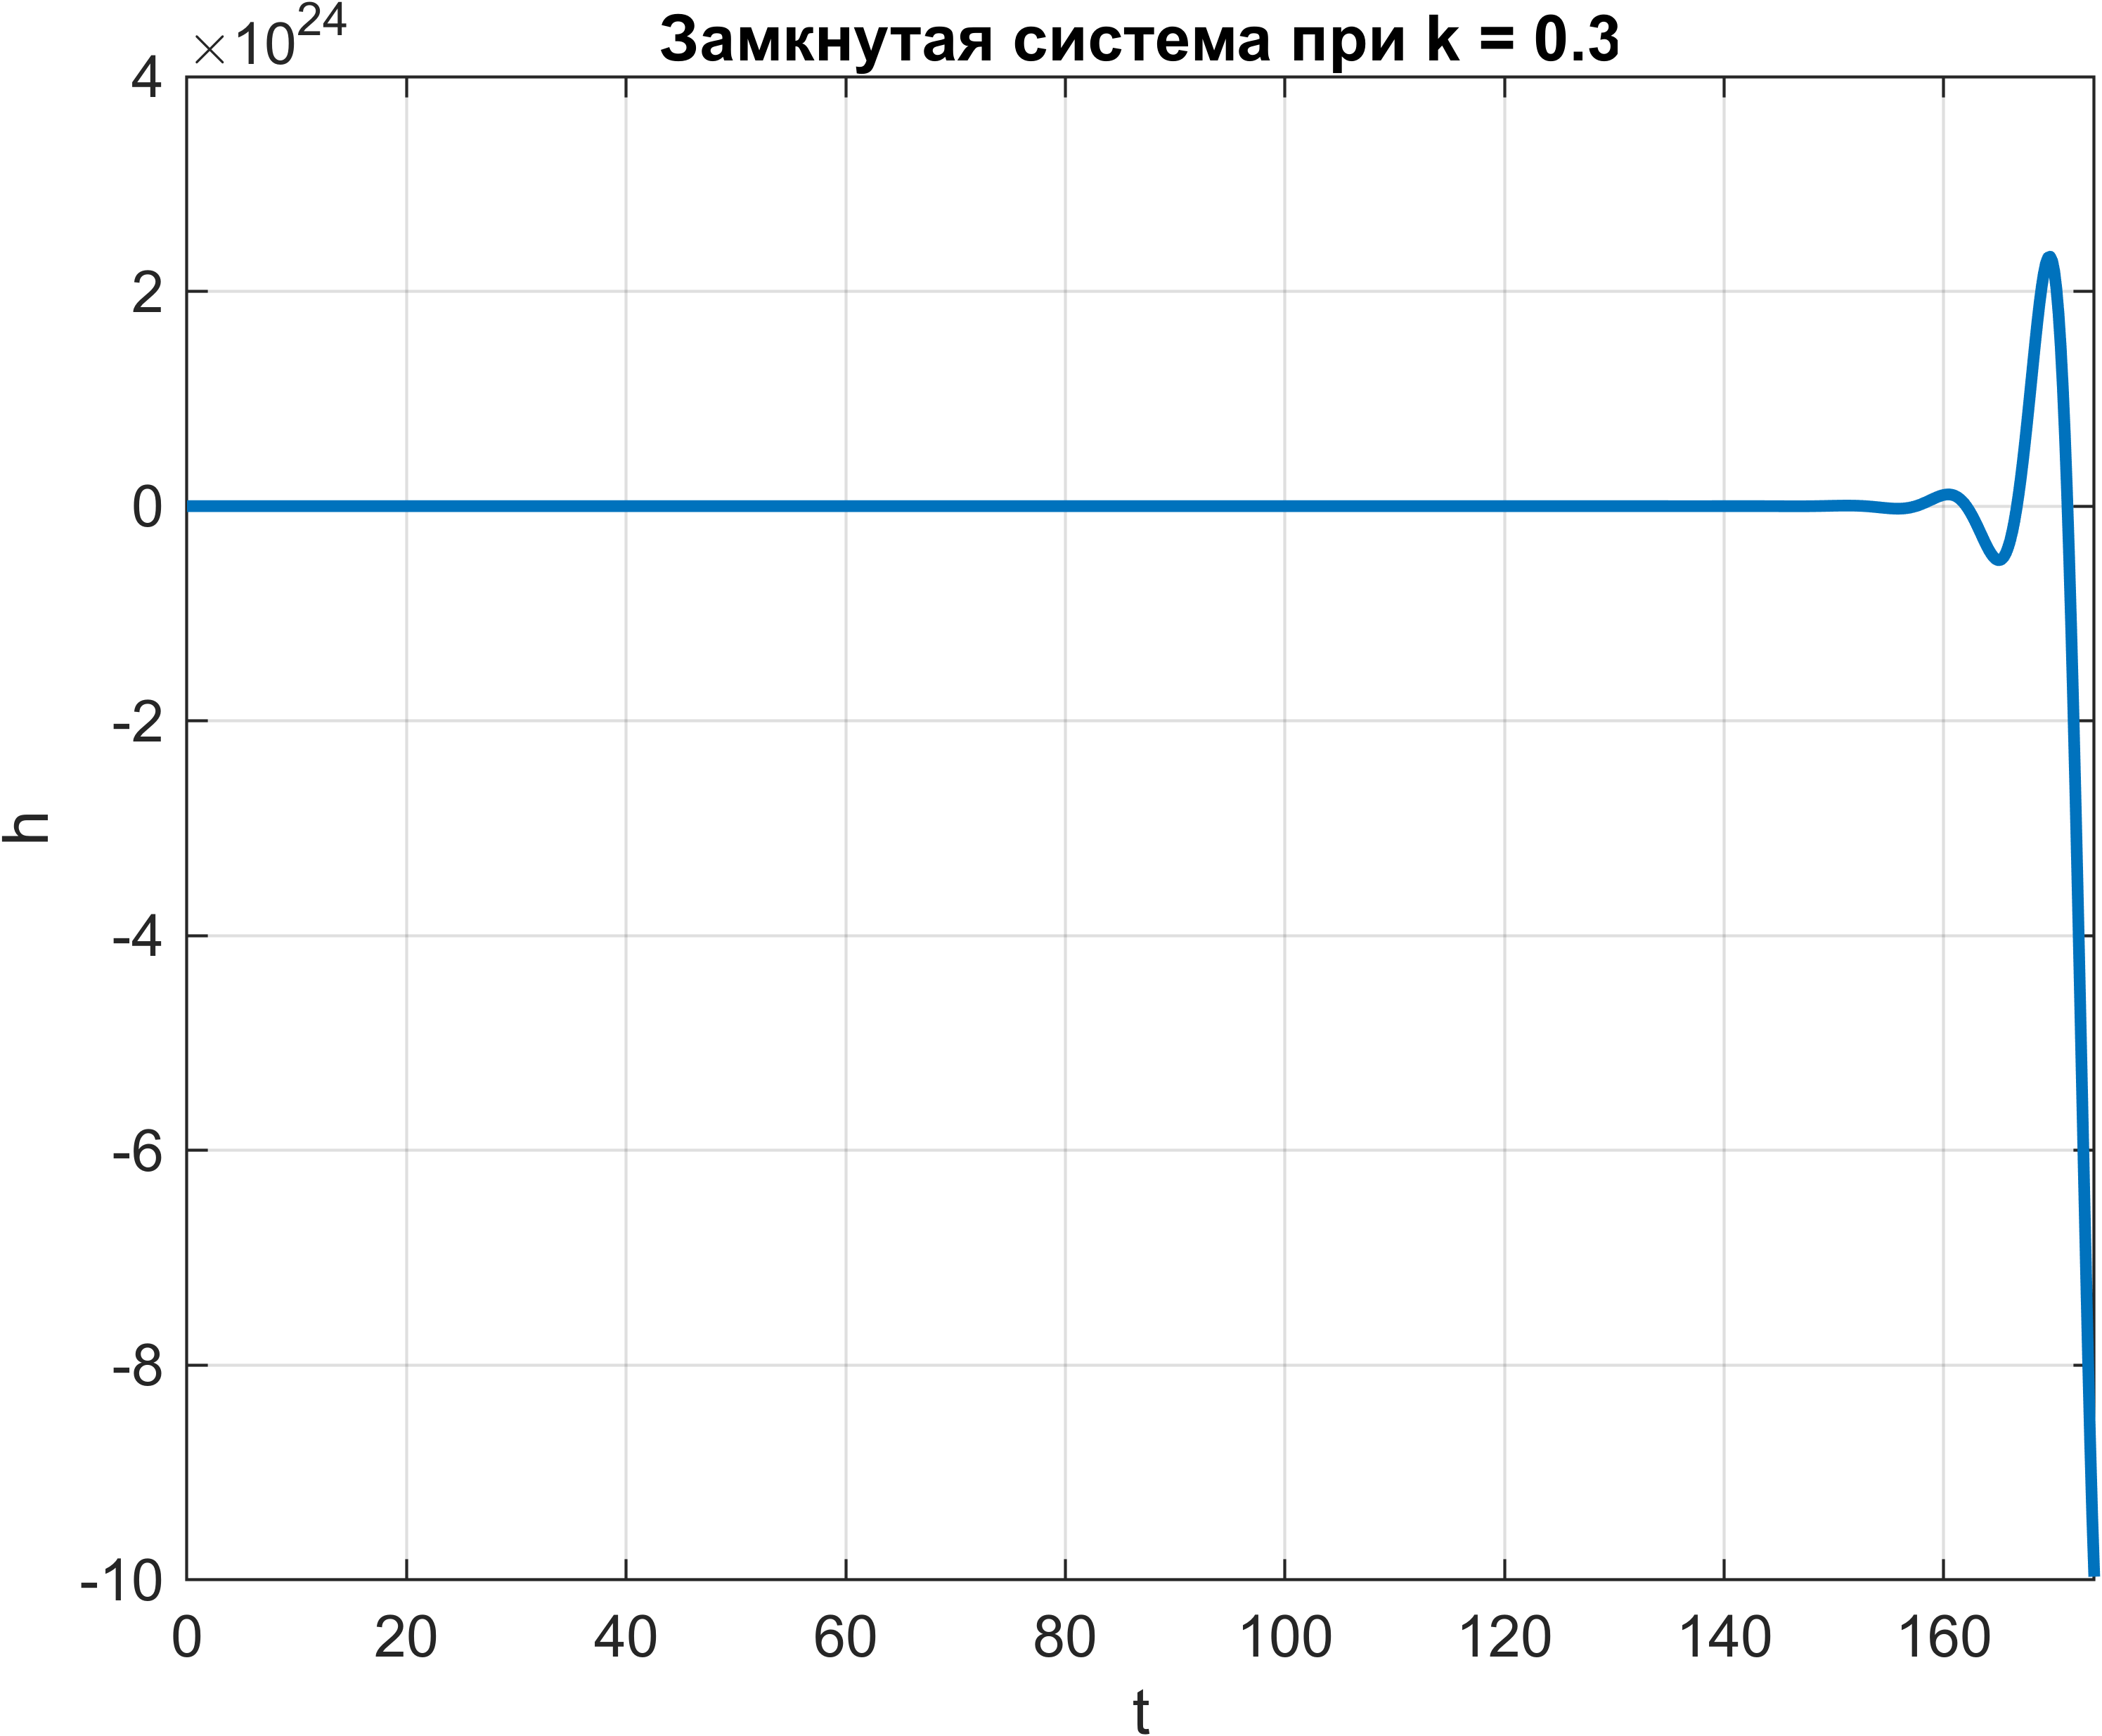
\includegraphics[width=1\textwidth, trim={0cm 0cm 0cm 0cm}]{../images/2_2_1_cl.png}
    \end{minipage}
    \hfill
    \begin{minipage}{0.45\textwidth}
        \centering
        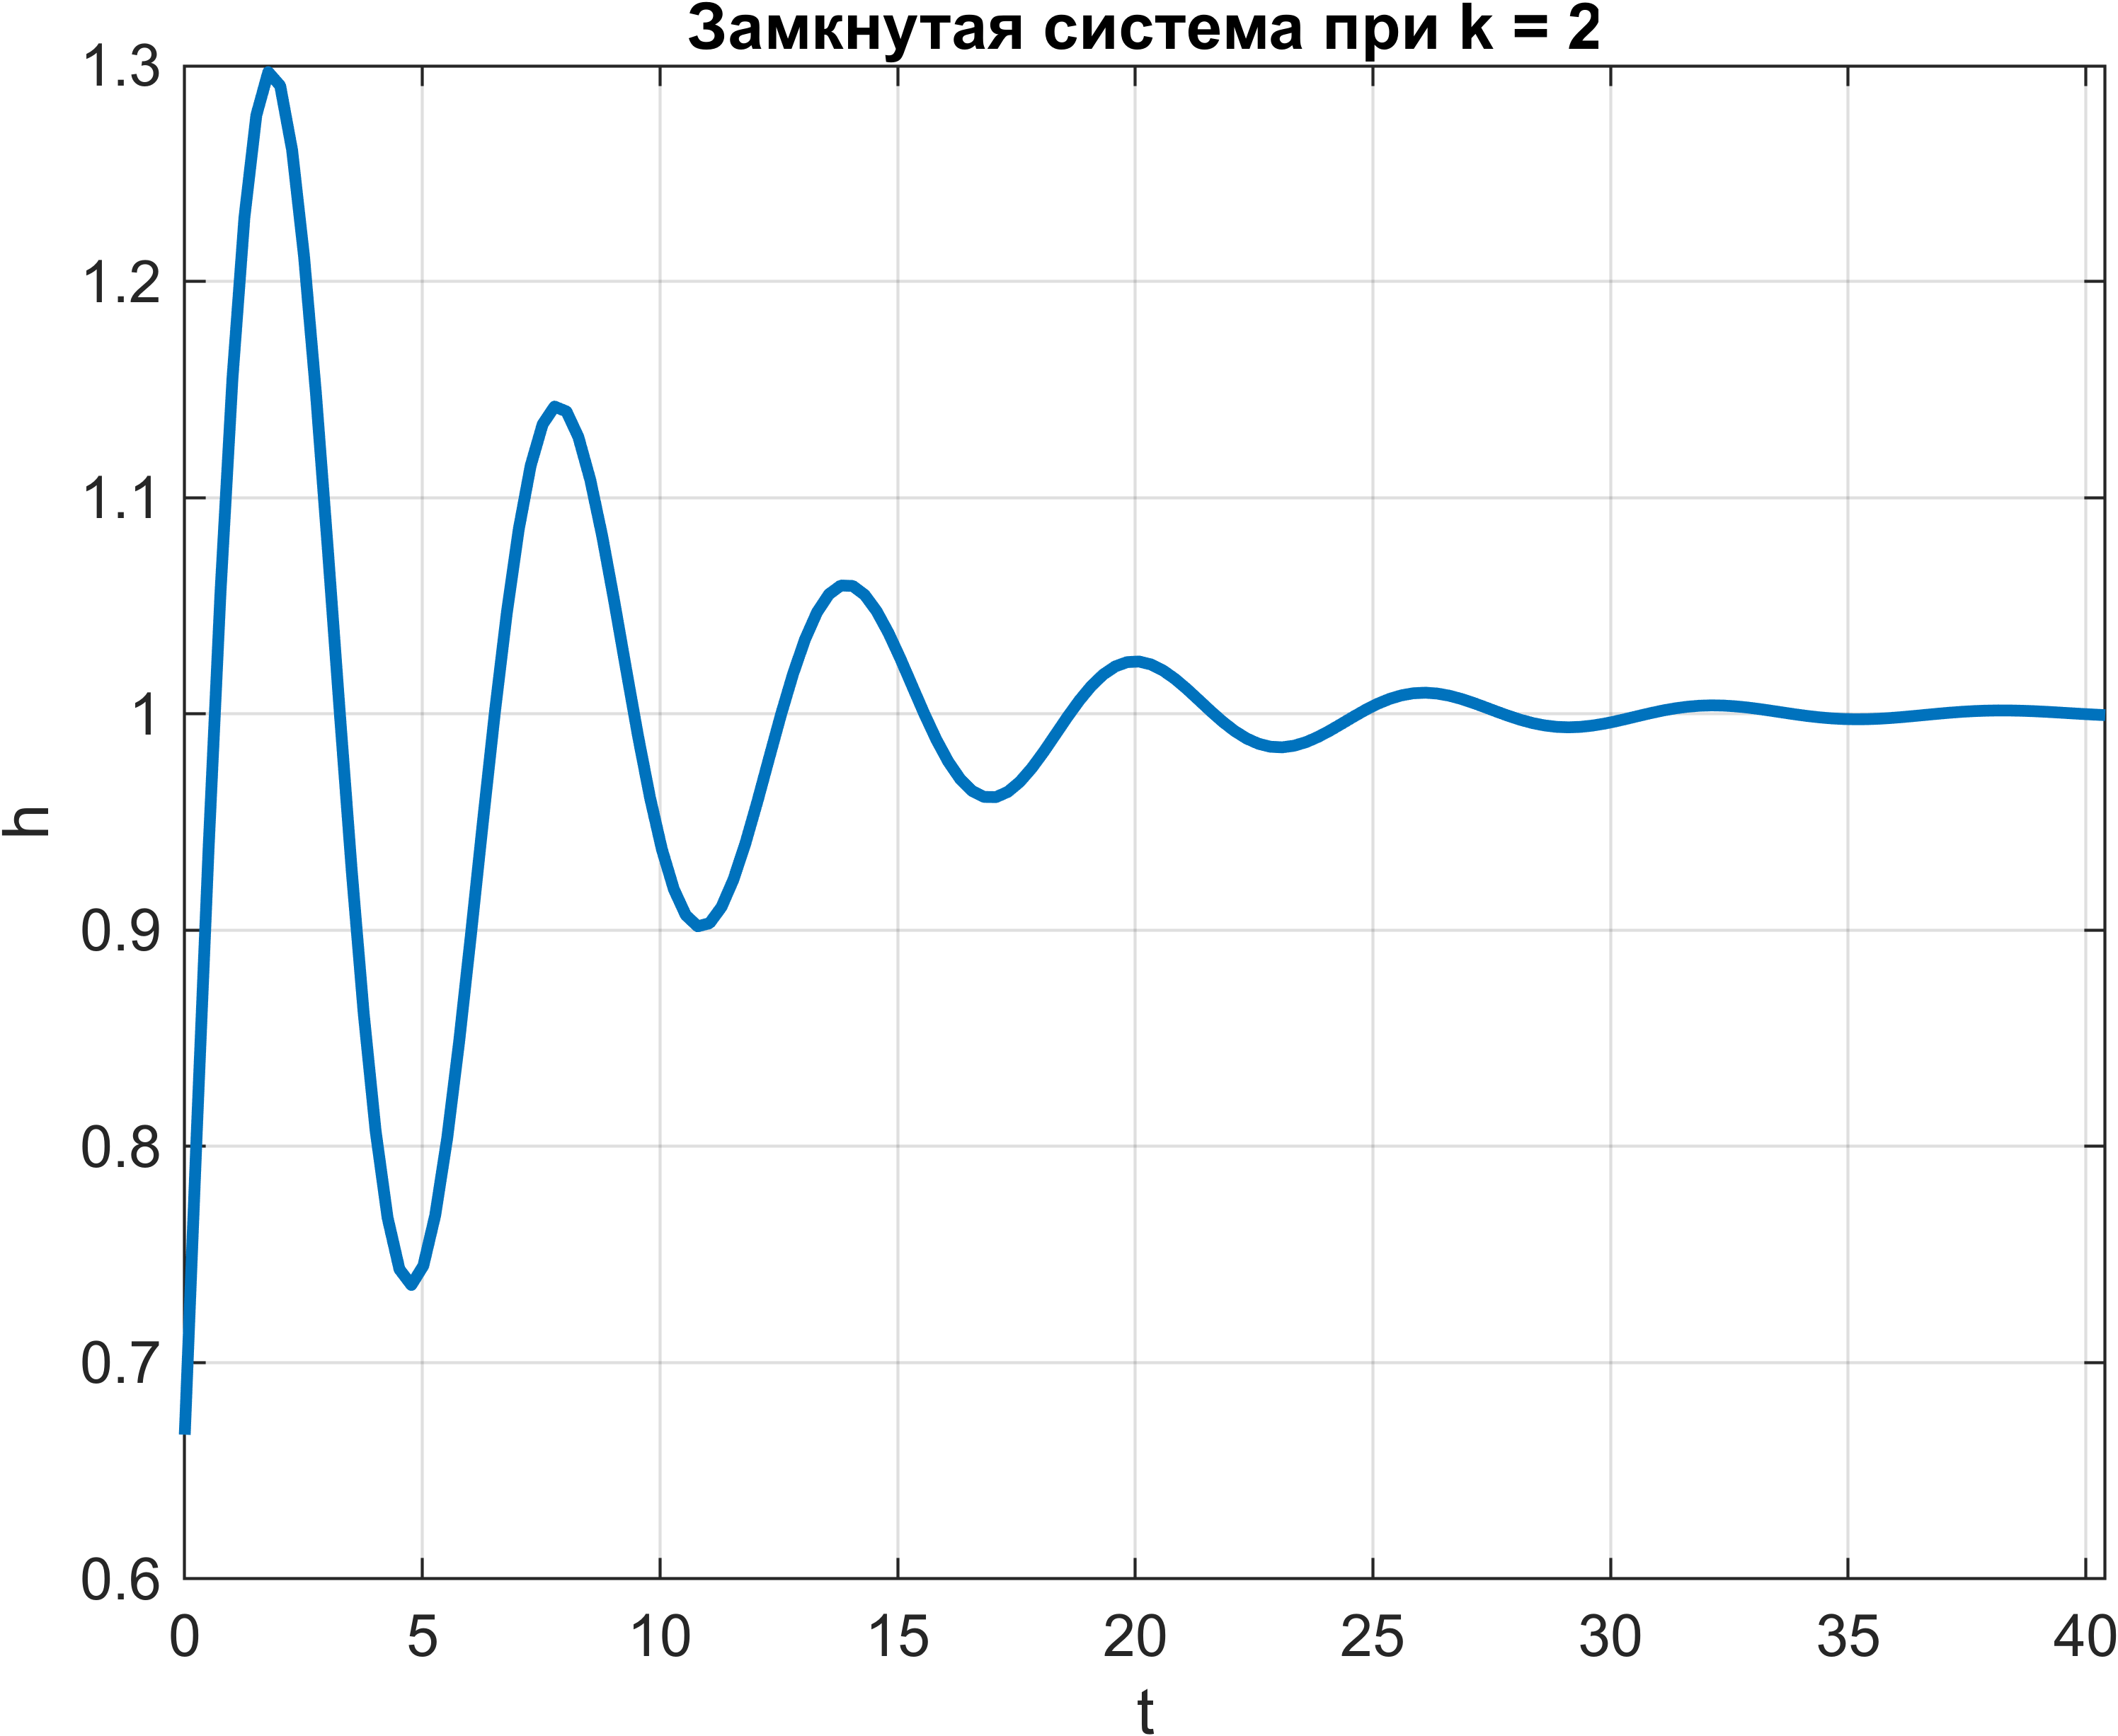
\includegraphics[width=1\textwidth, trim={0cm 0cm 0cm 0cm}]{../images/2_2_2_cl.png}
    \end{minipage}
    \caption{Переходные характеристики системы при $k = 0.3$ и $k = 2$}
\end{figure}
\endinput
